\section{Porównanie działania modeli linowych z działaniem modelu nieliniowego}

Poniżej przedstawione wykresy są rezultatem wprowadzenia wyprowadzonych równań stanu do Matlaba 


W pierwszym eksperymencie sprawdzono działanie modelu dla różnych wartości wejścia $u_1$ pozostawiając wartości $u_2$ i $v_1$ stałe w punkcie pracy.

\begin{figure}[H]
    \centering
    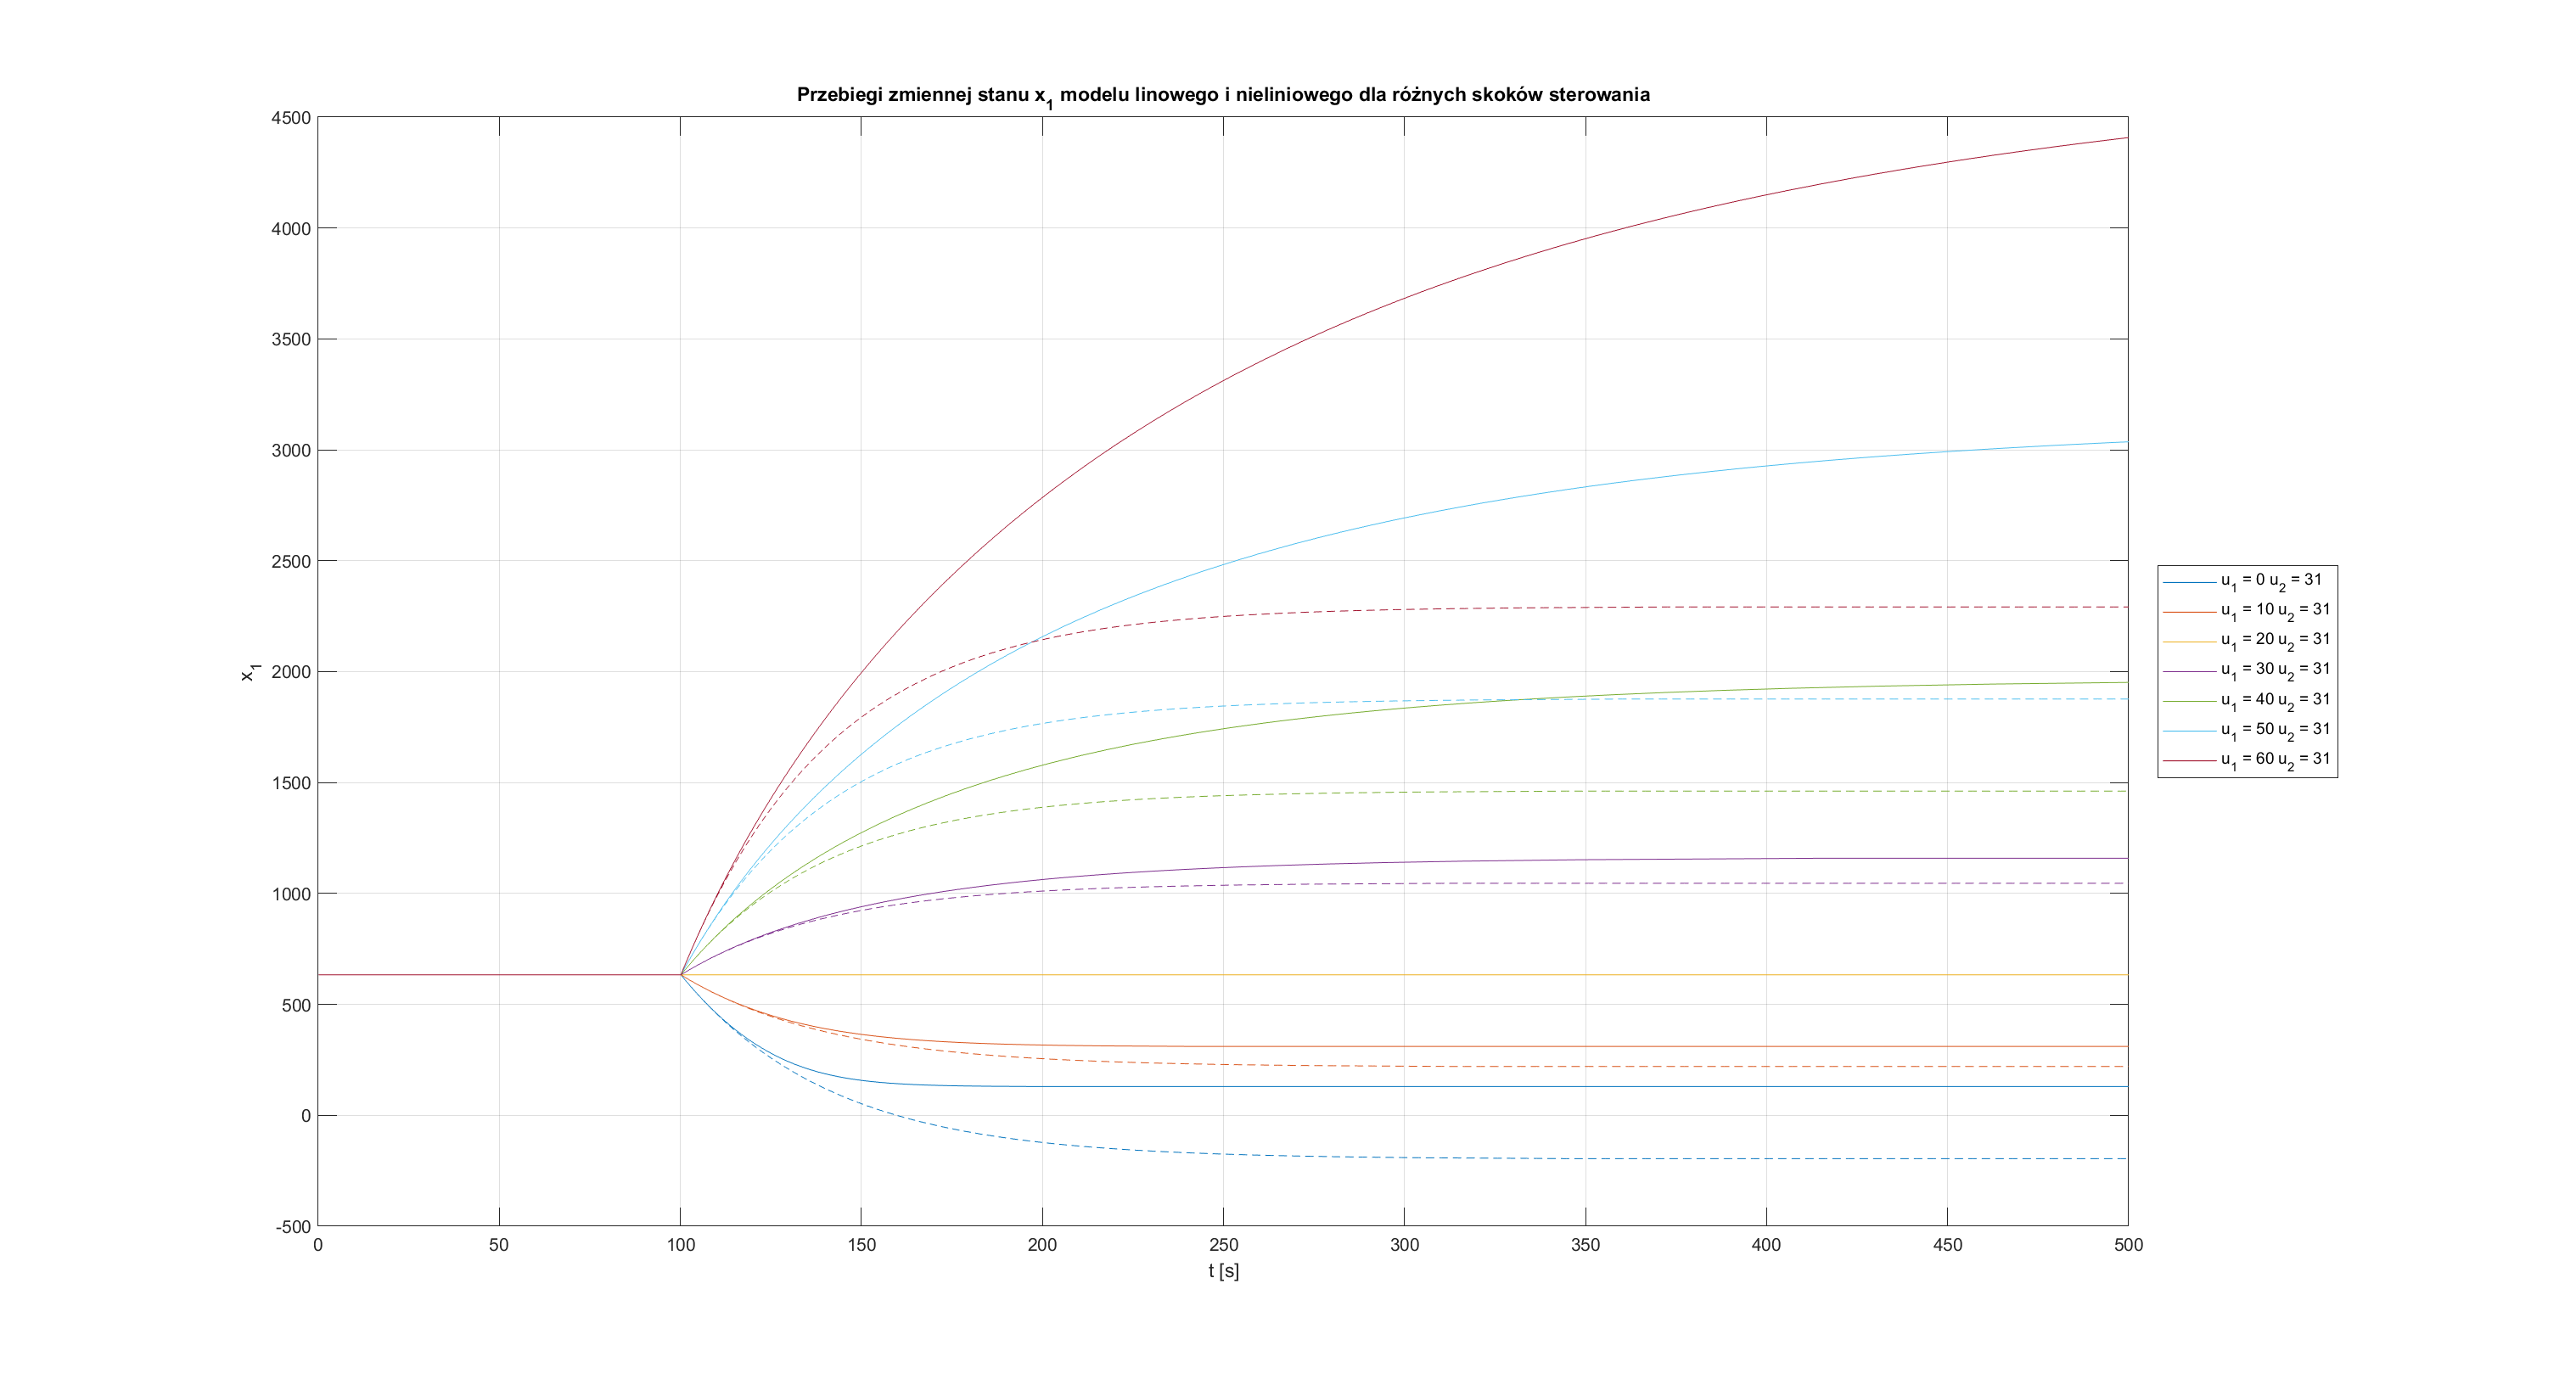
\includegraphics[scale=0.35]{images/x1_u1=60_u2=31_dt=0.1.eps}
    \caption{Porównanie modeli liniowych i nieliniowych}
\end{figure}

\begin{figure}[H]
    \centering
    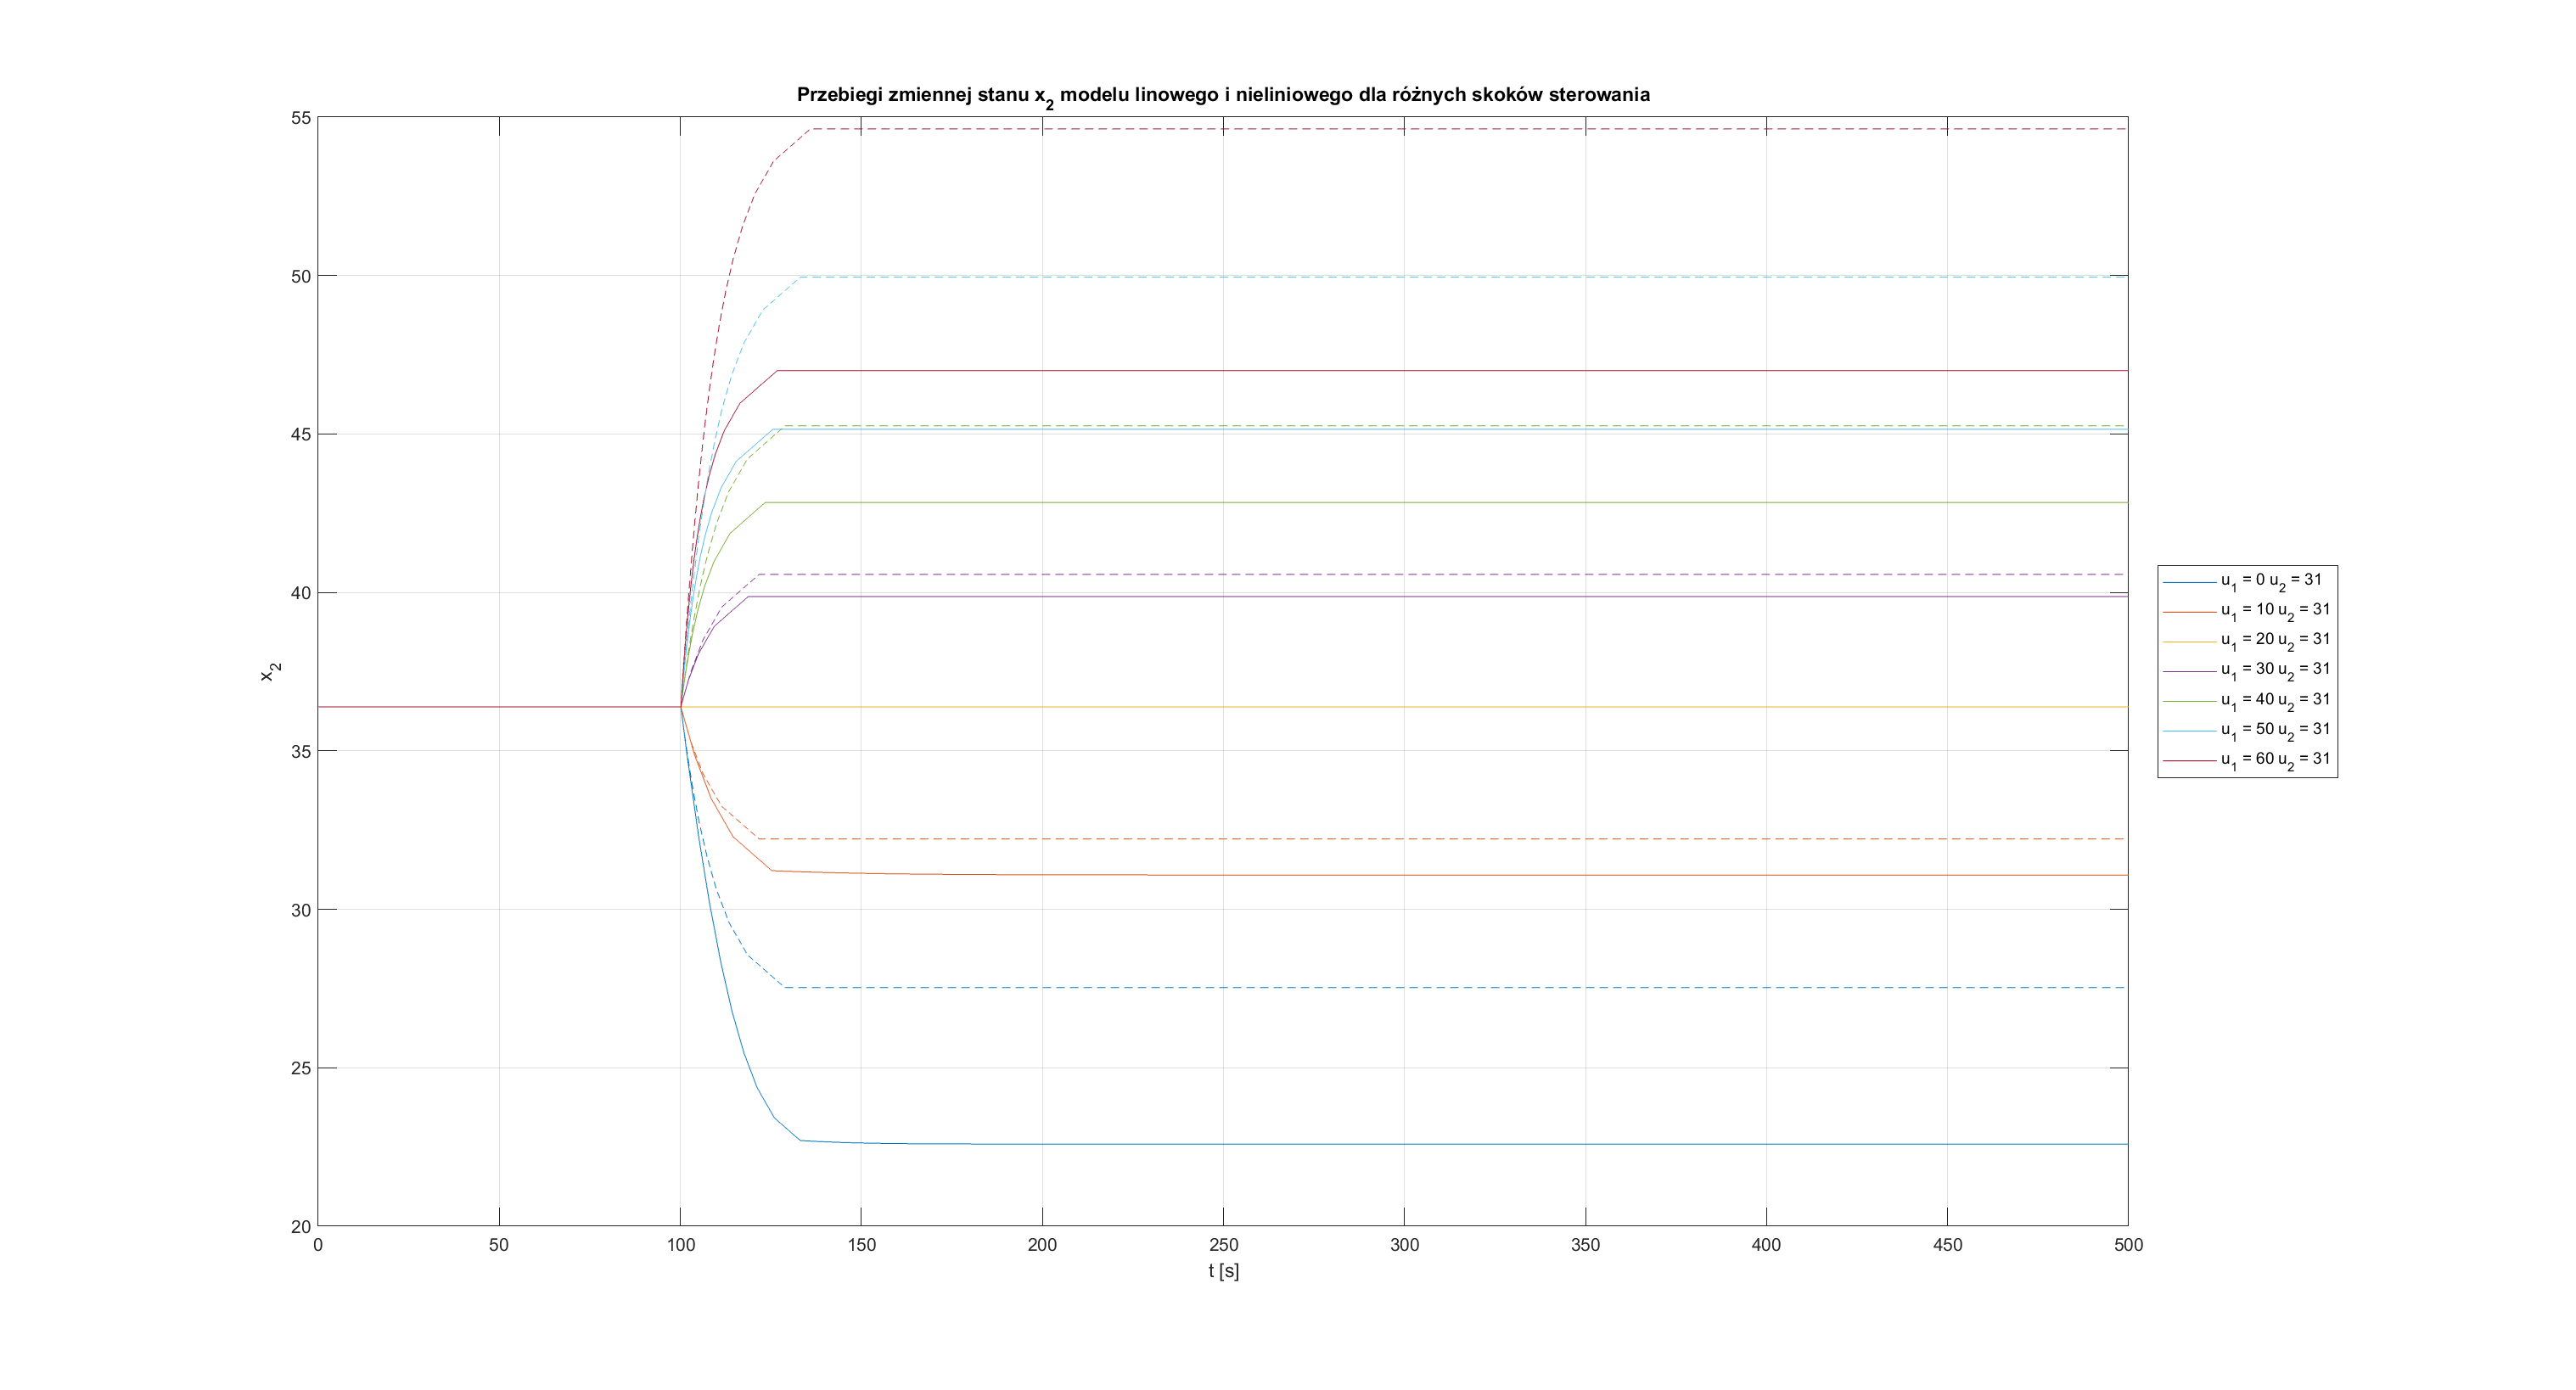
\includegraphics[scale=0.35]{images/x2_u1=60_u2=31_dt=0.1.eps}
    \caption{Porównanie modeli liniowych i nieliniowych}
\end{figure}

\begin{figure}[H]
    \centering
    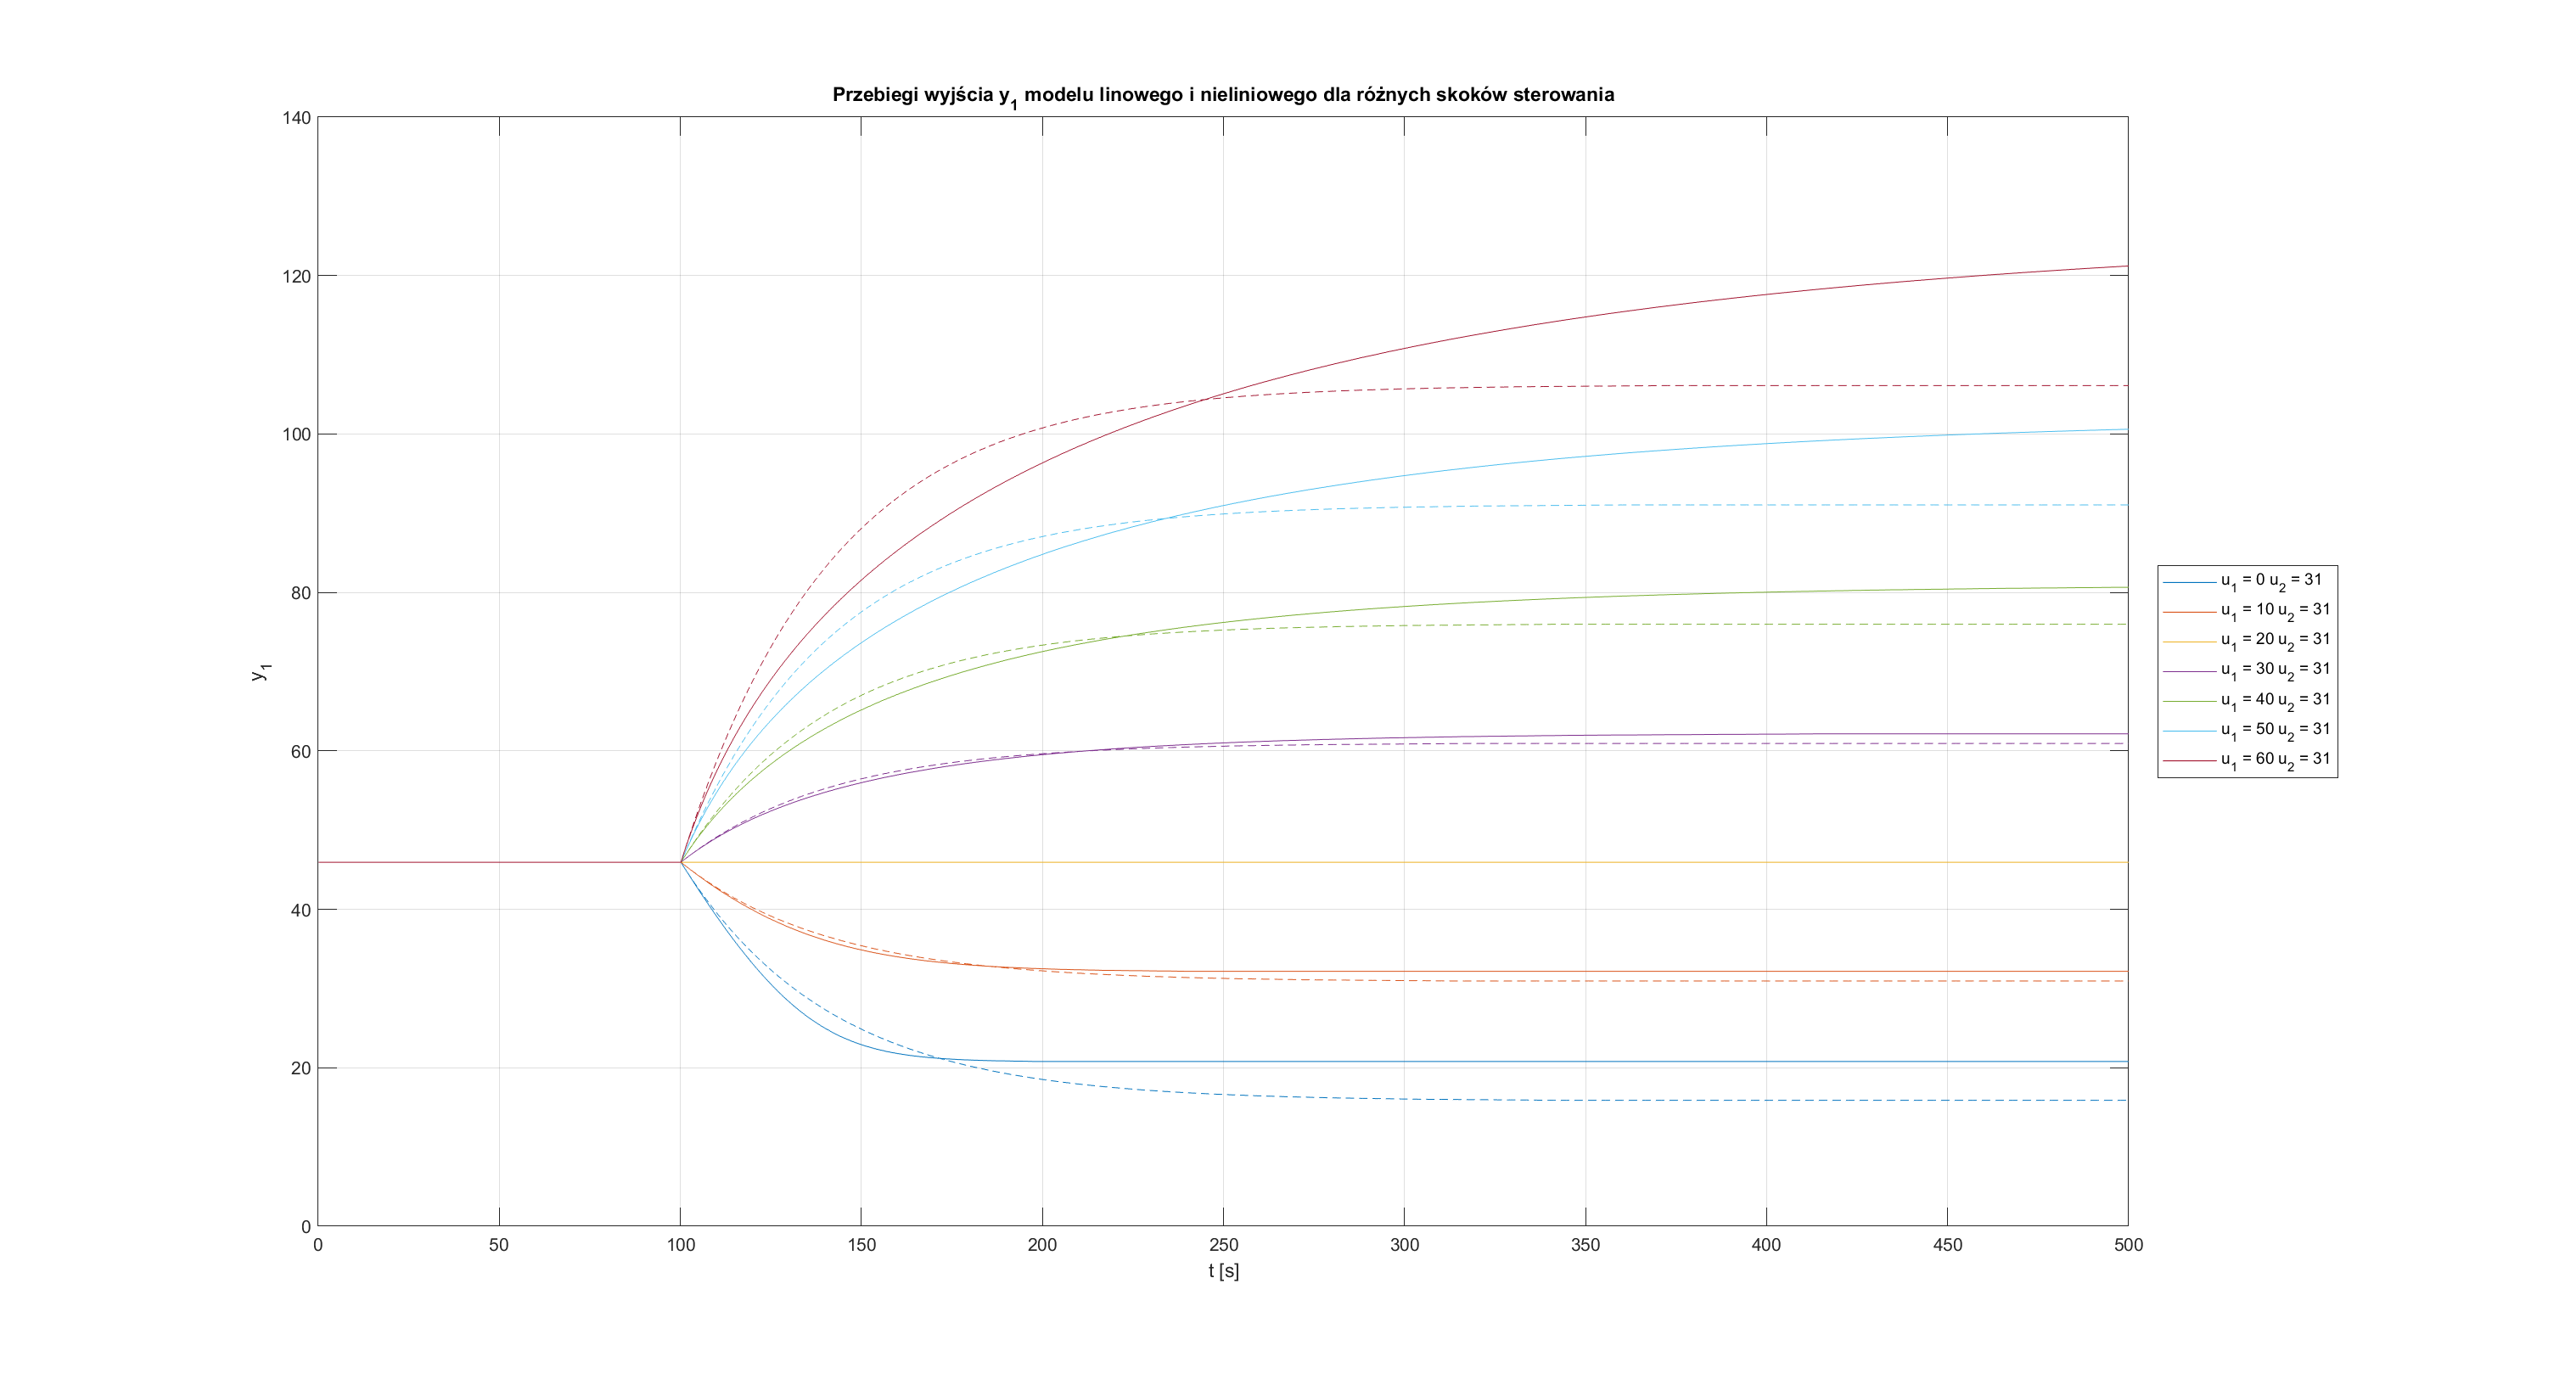
\includegraphics[scale=0.35]{images/y1_u1=60_u2=31_dt=0.1.eps}
    \caption{Porównanie modeli liniowych i nieliniowych}
\end{figure}

\begin{figure}[H]
    \centering
    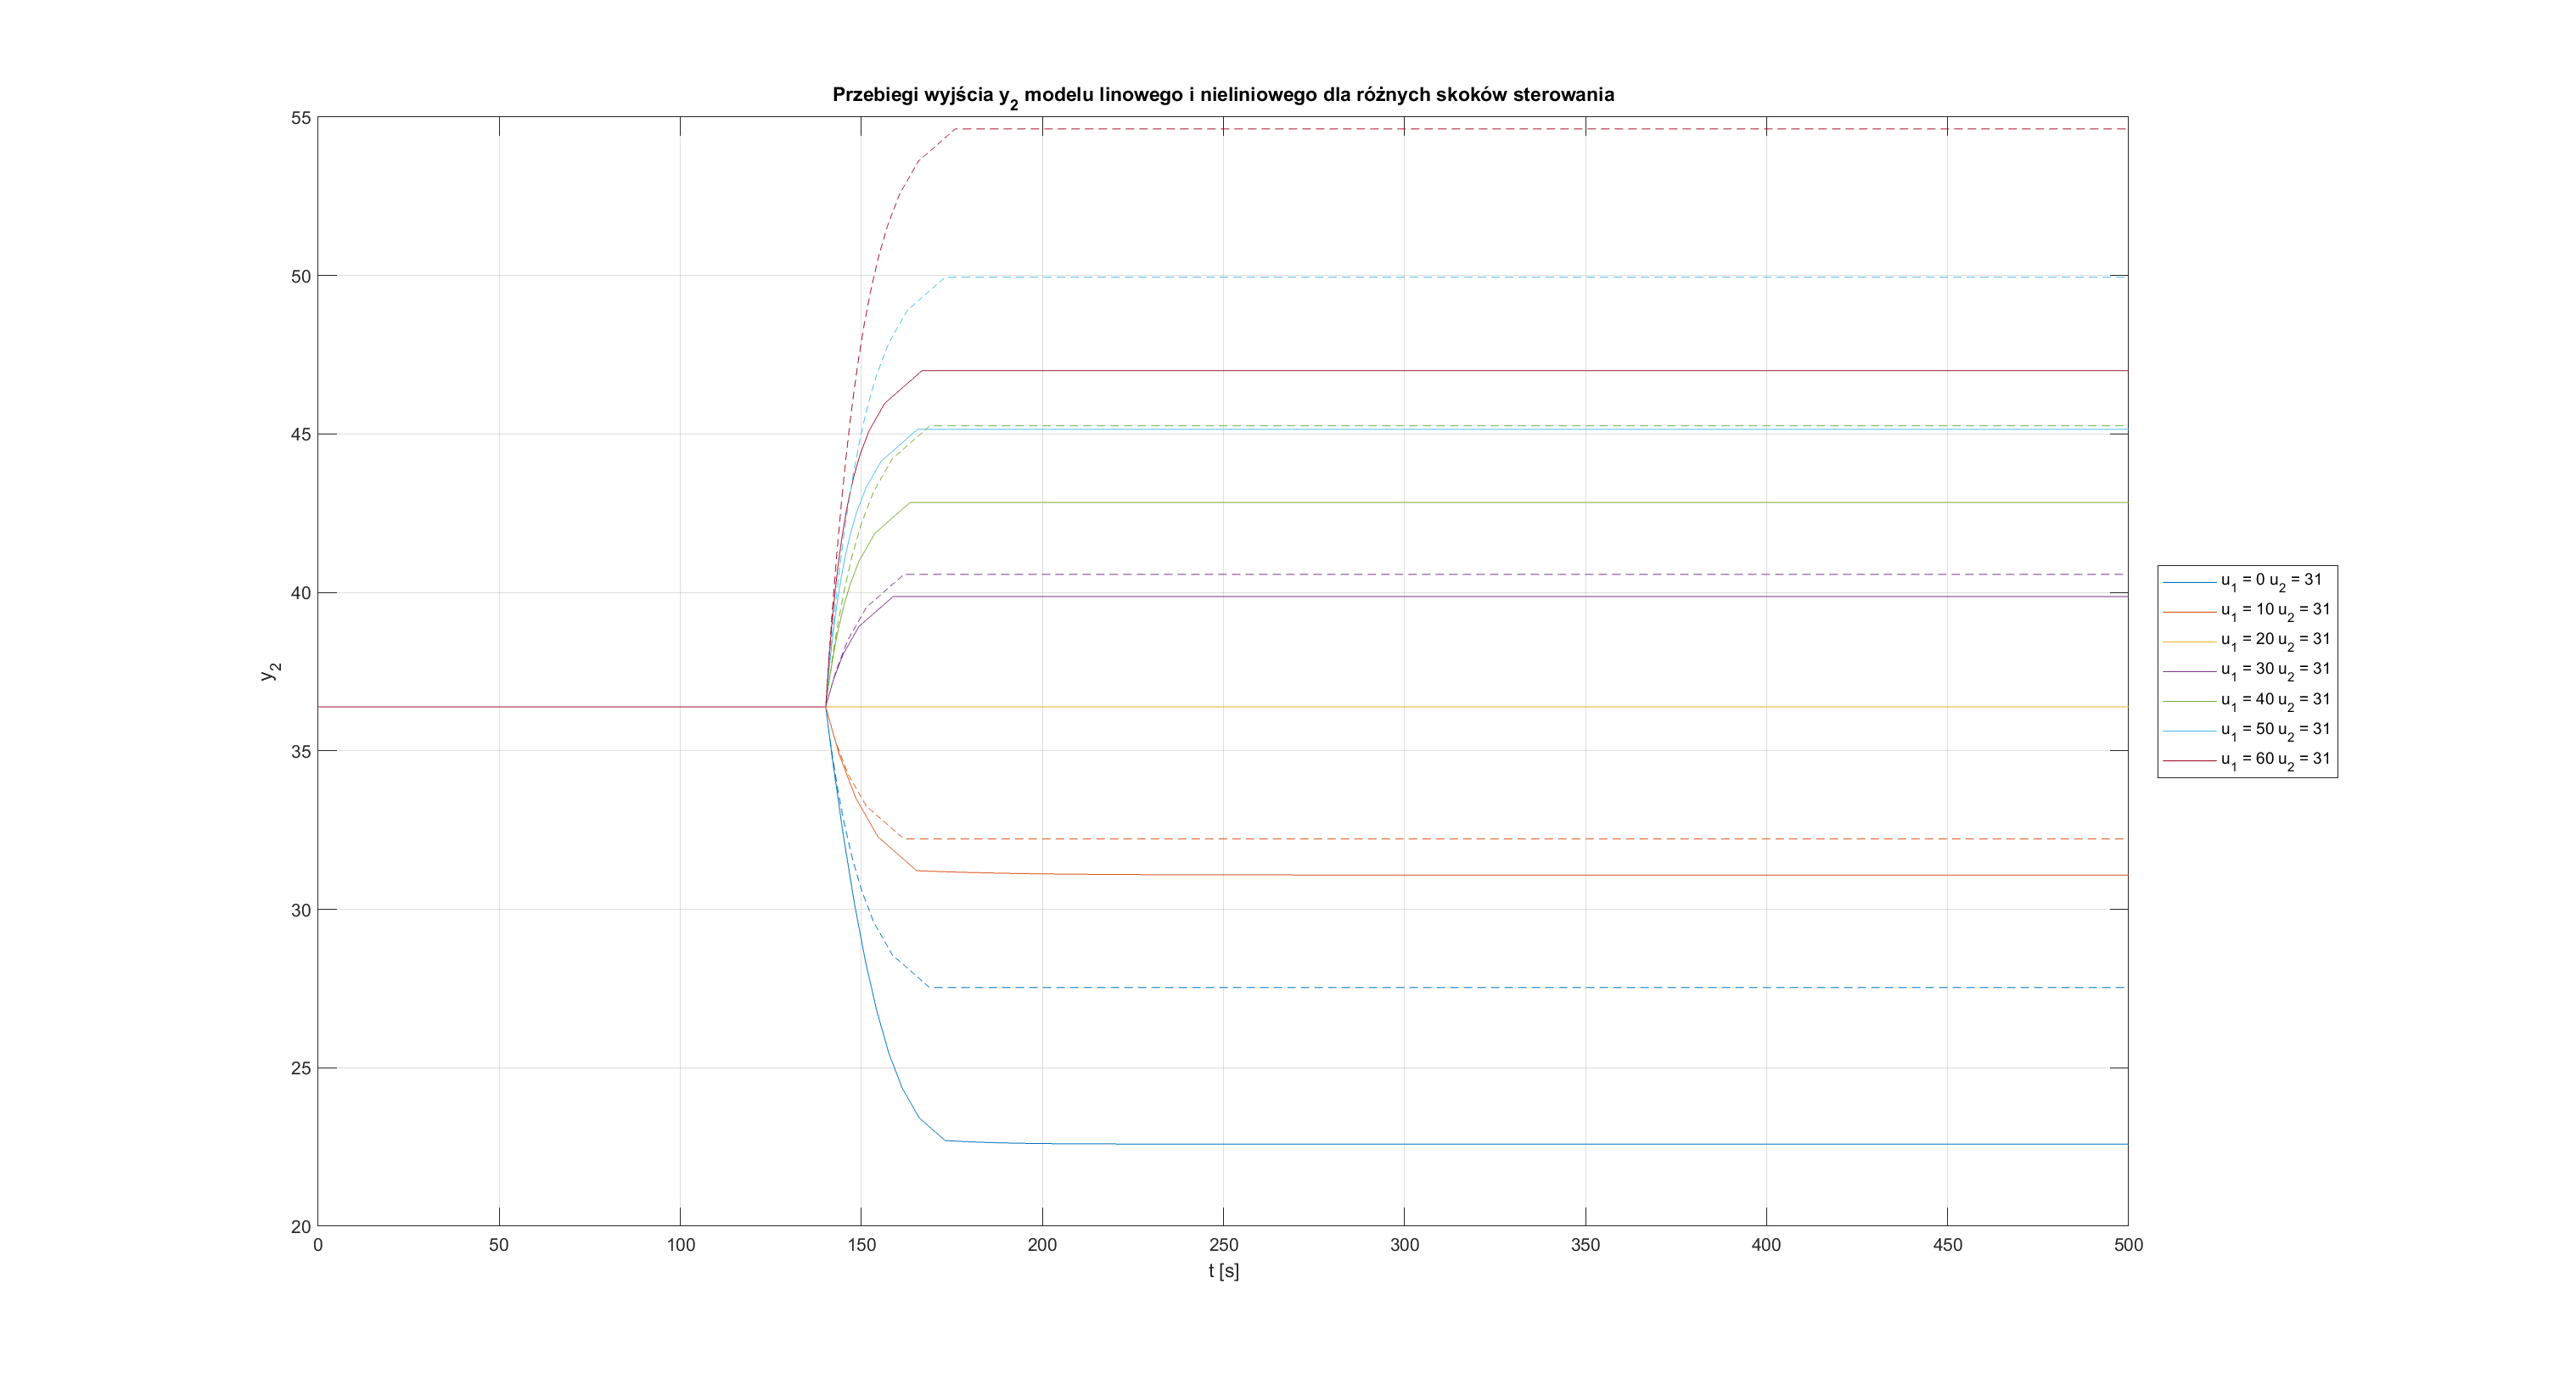
\includegraphics[scale=0.35]{images/y2_u1=60_u2=31_dt=0.1.eps}
    \caption{Porównanie modeli liniowych i nieliniowych}
\end{figure}

W kolejnym sprawdzano zachowanie układu dla różnych wartości $u_2$, resztę pozostawiając bez zmian.

\begin{figure}[H]
    \centering
    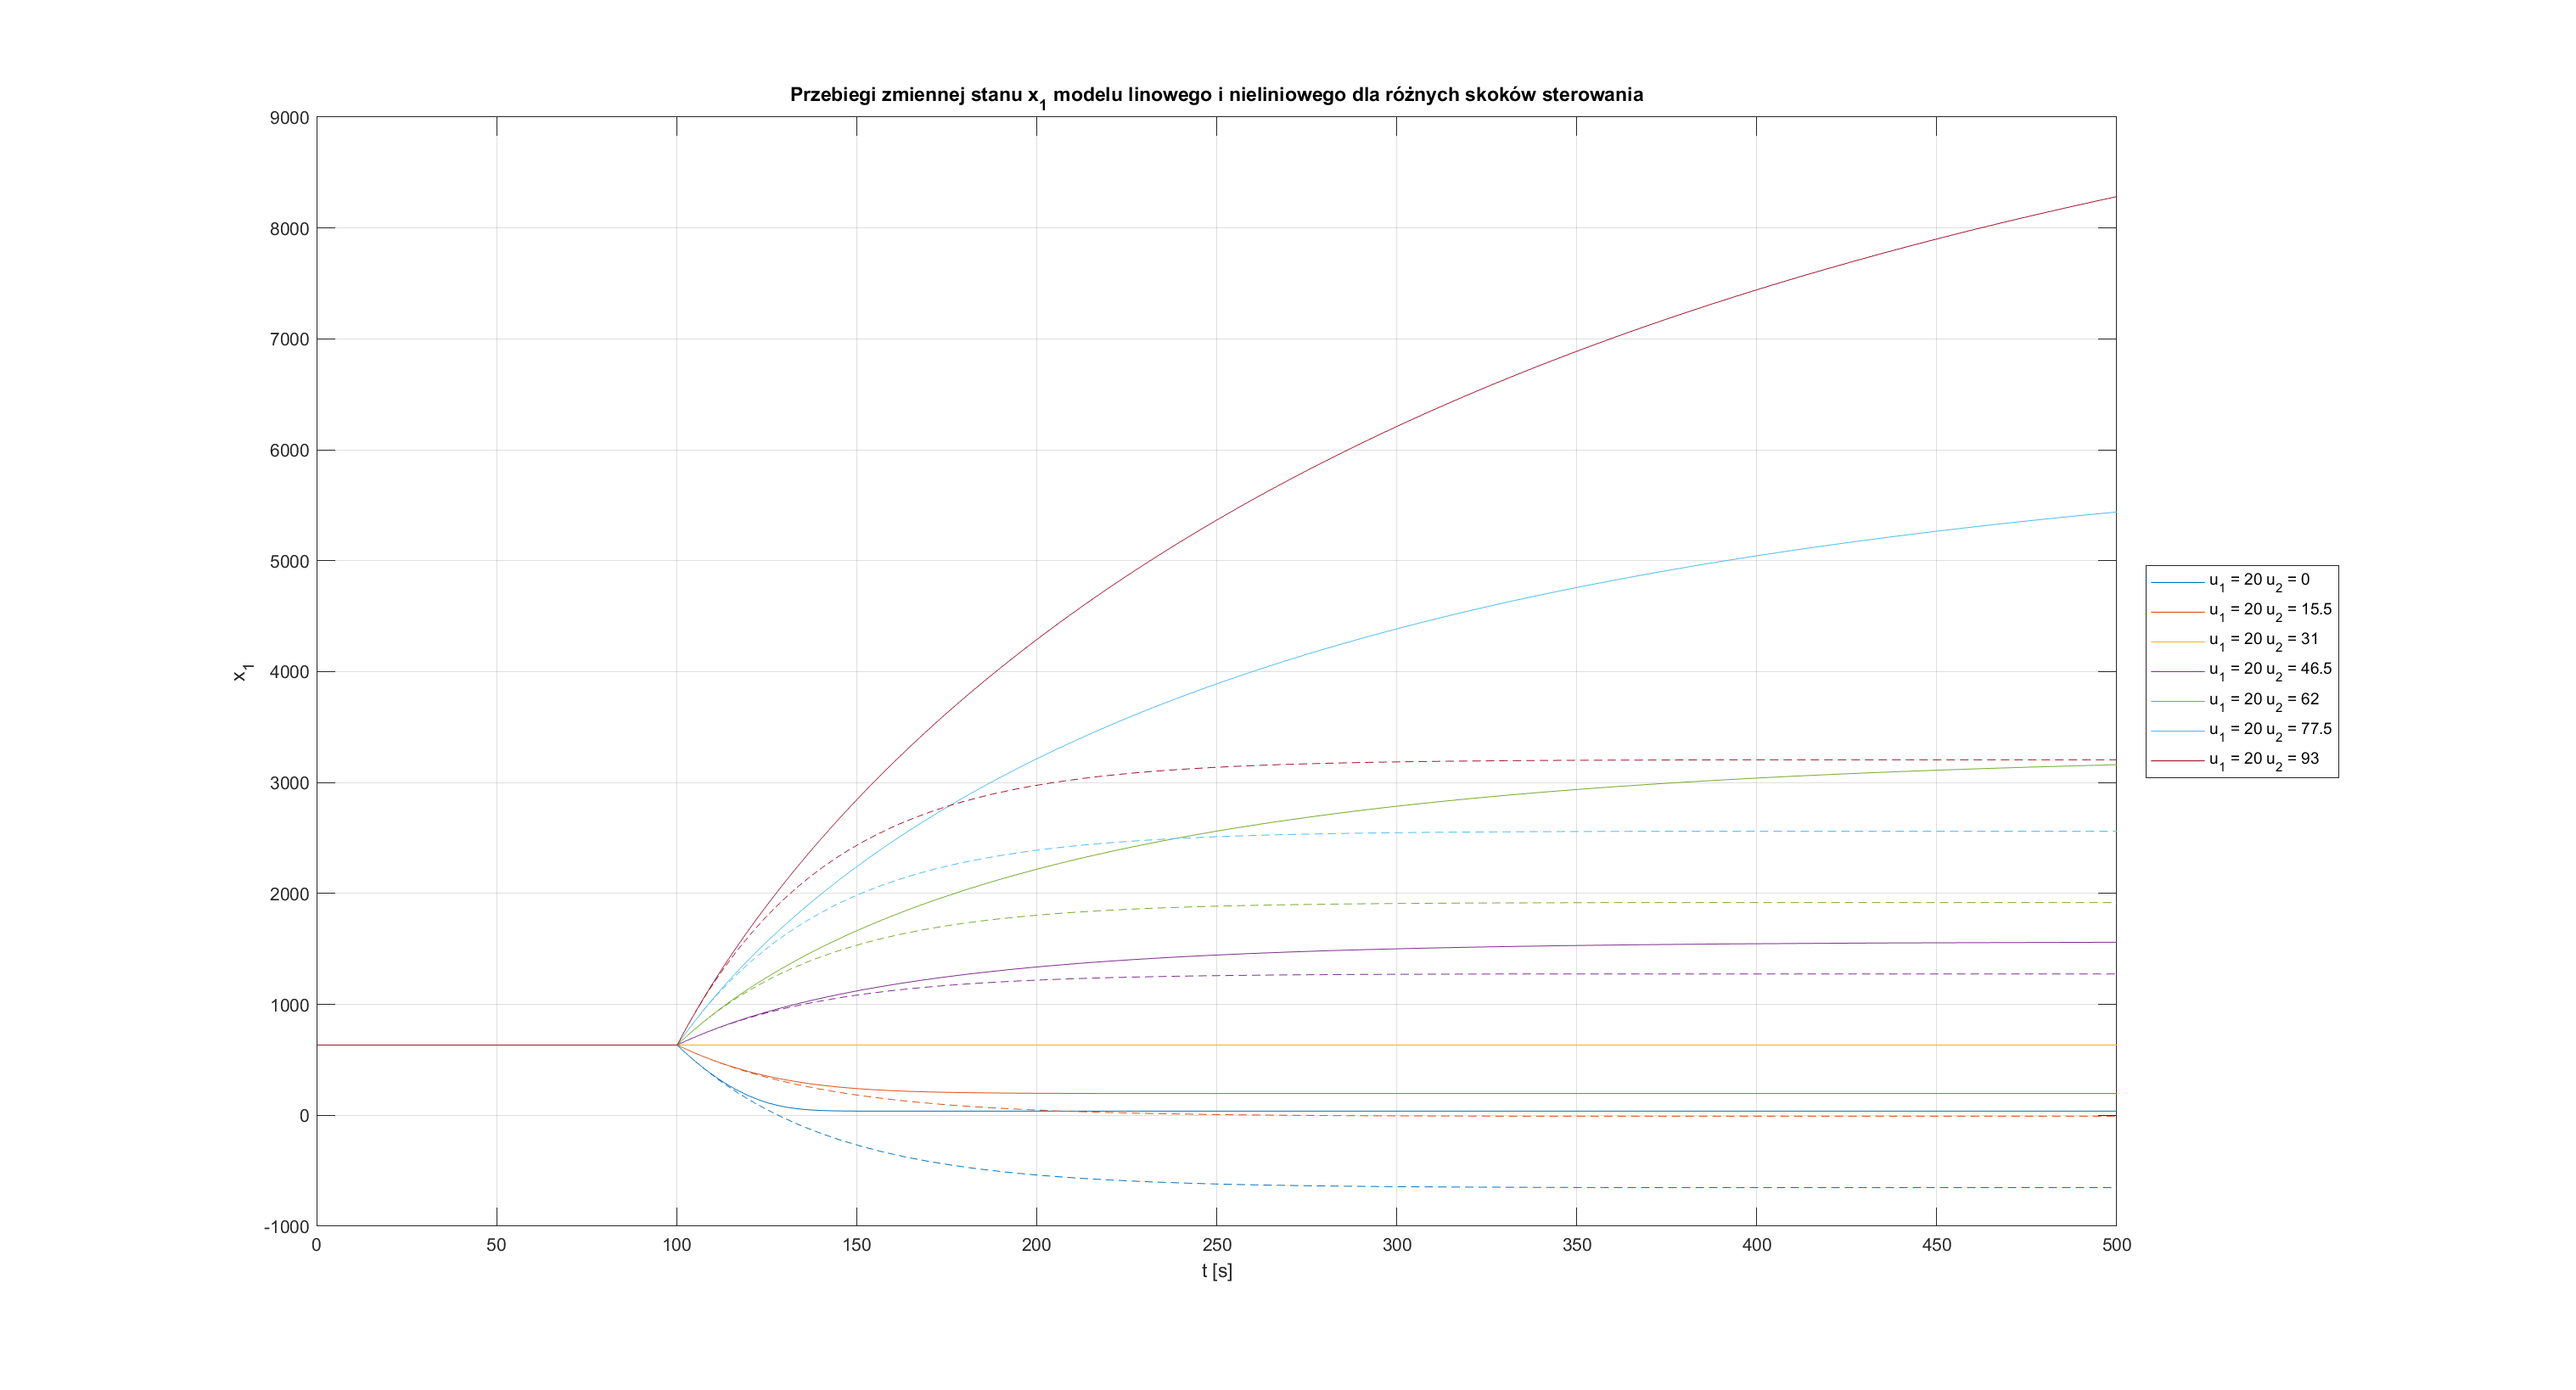
\includegraphics[scale=0.35]{images/x1_u1=20_u2=93_dt=0.1.eps}
    \caption{Porównanie modeli liniowych i nieliniowych}
\end{figure}

\begin{figure}[H]
    \centering
    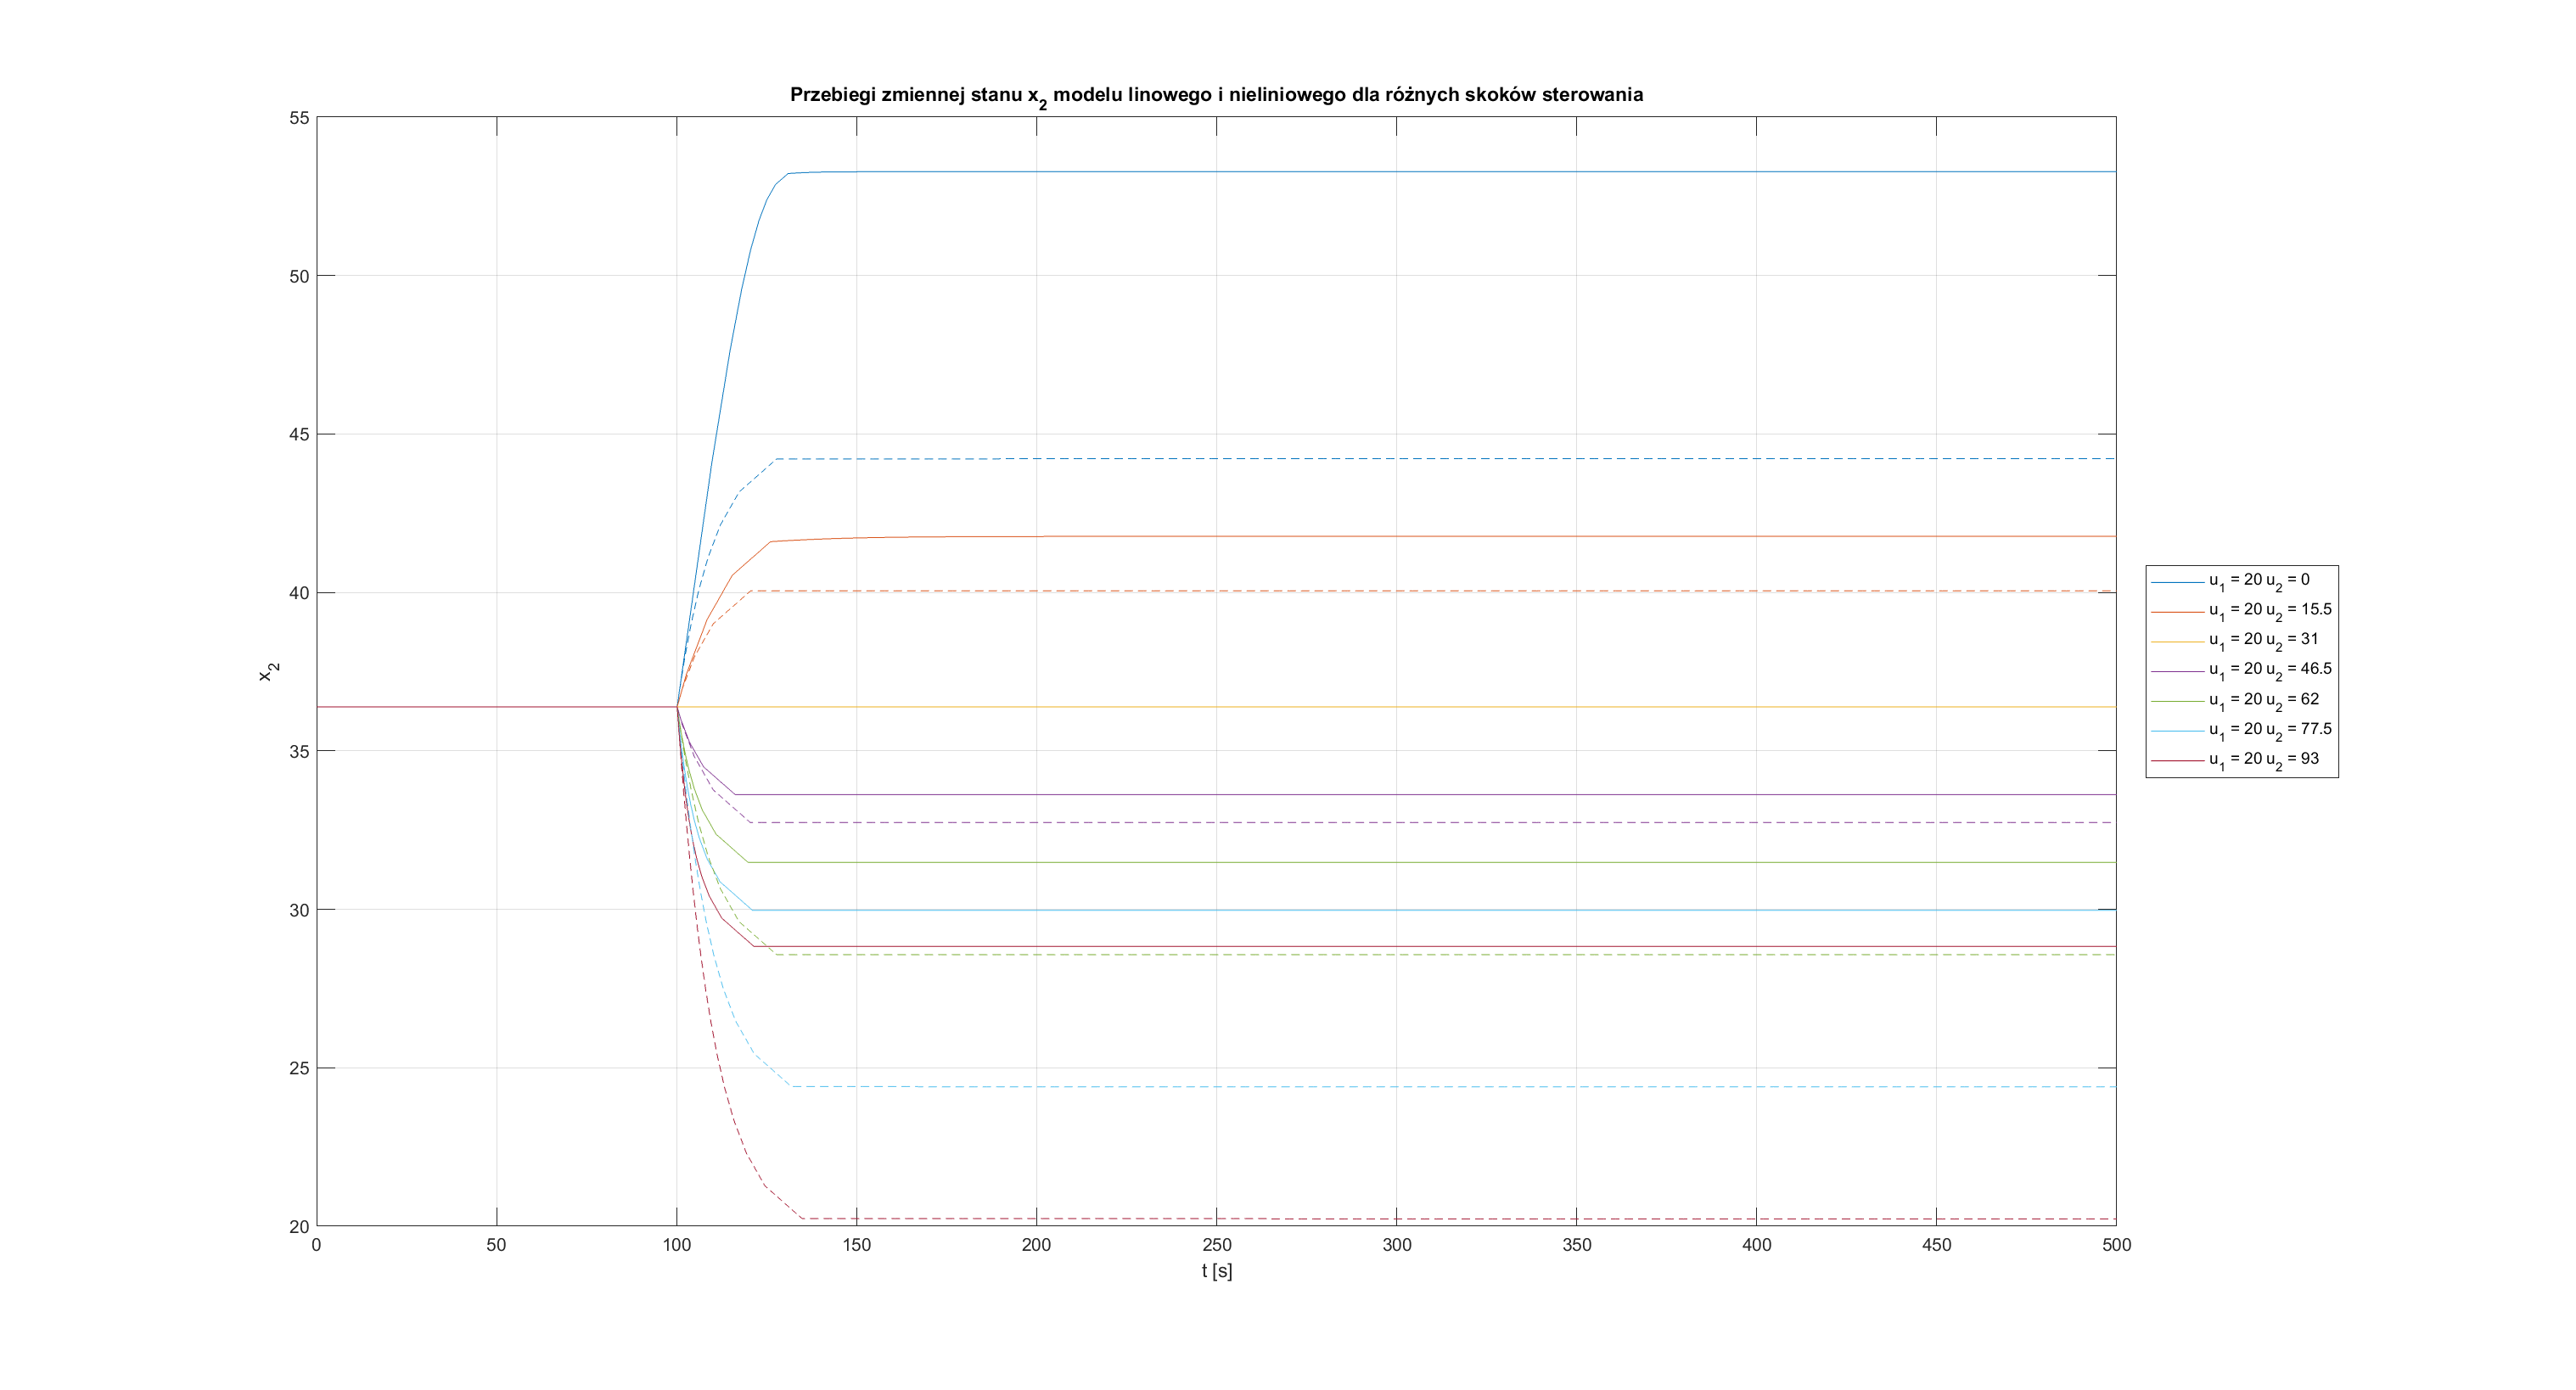
\includegraphics[scale=0.35]{images/x2_u1=20_u2=93_dt=0.1.eps}
    \caption{Porównanie modeli liniowych i nieliniowych}
\end{figure}

\begin{figure}[H]
    \centering
    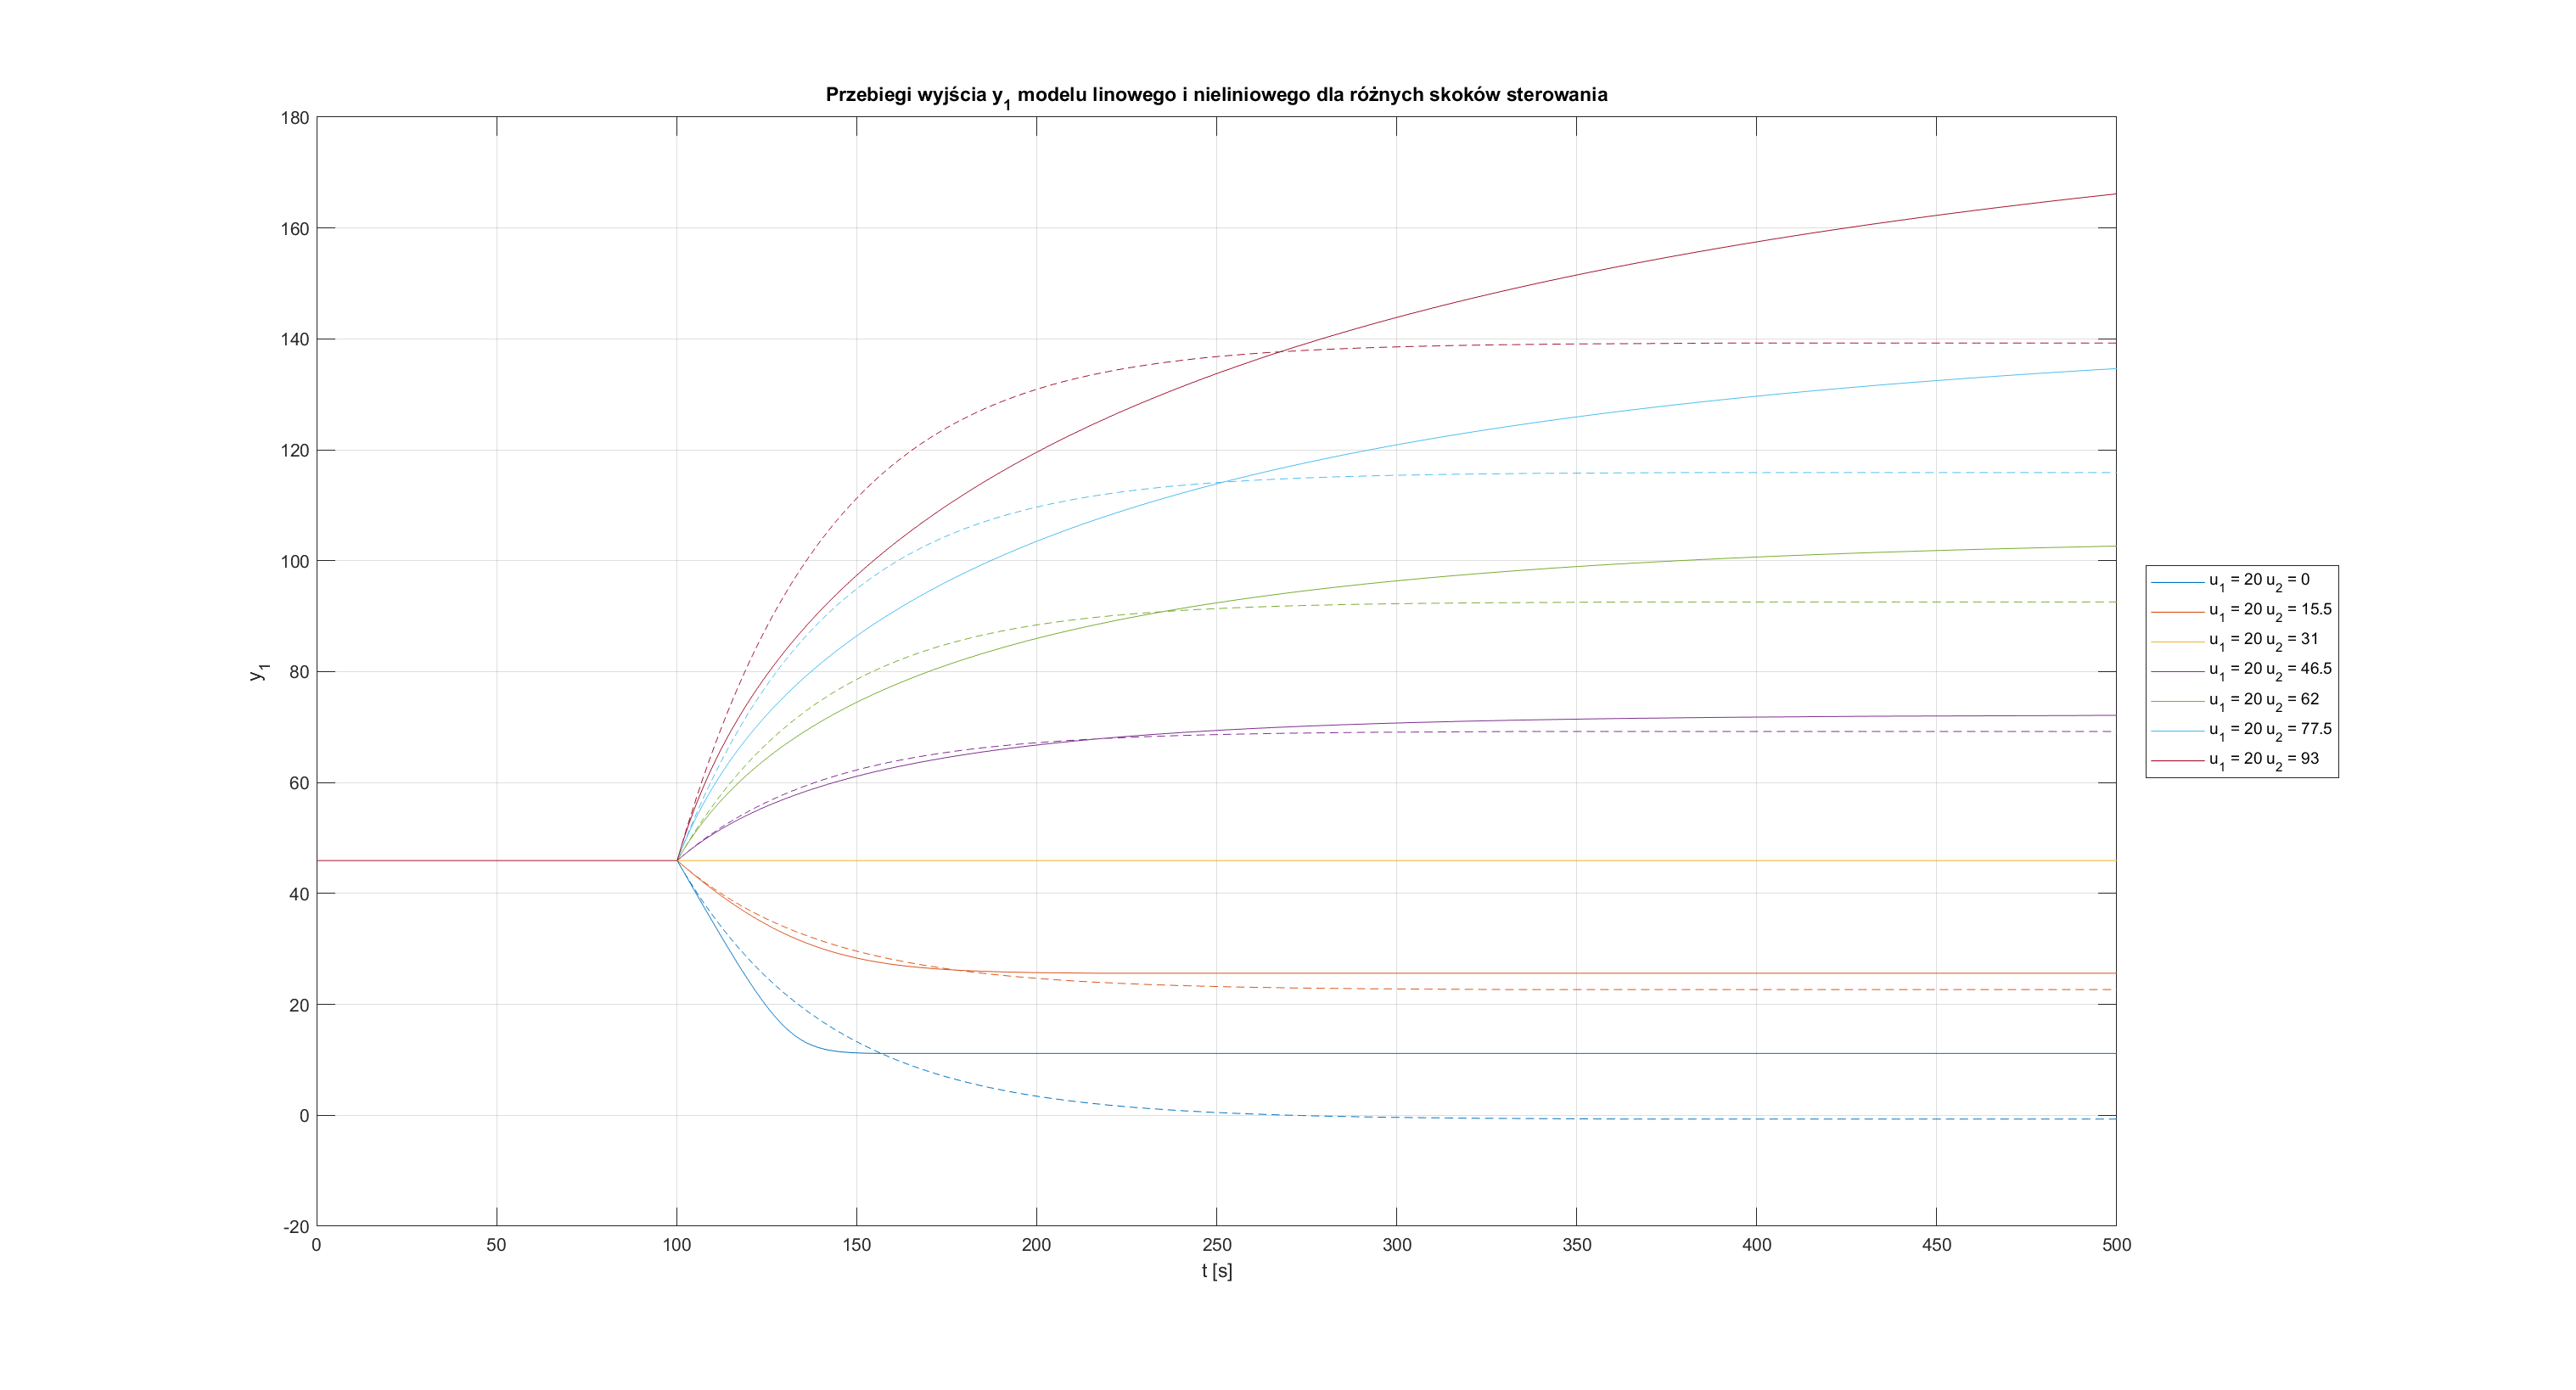
\includegraphics[scale=0.35]{images/y1_u1=20_u2=93_dt=0.1.eps}
    \caption{Porównanie modeli liniowych i nieliniowych}
\end{figure}

\begin{figure}[H]
    \centering
    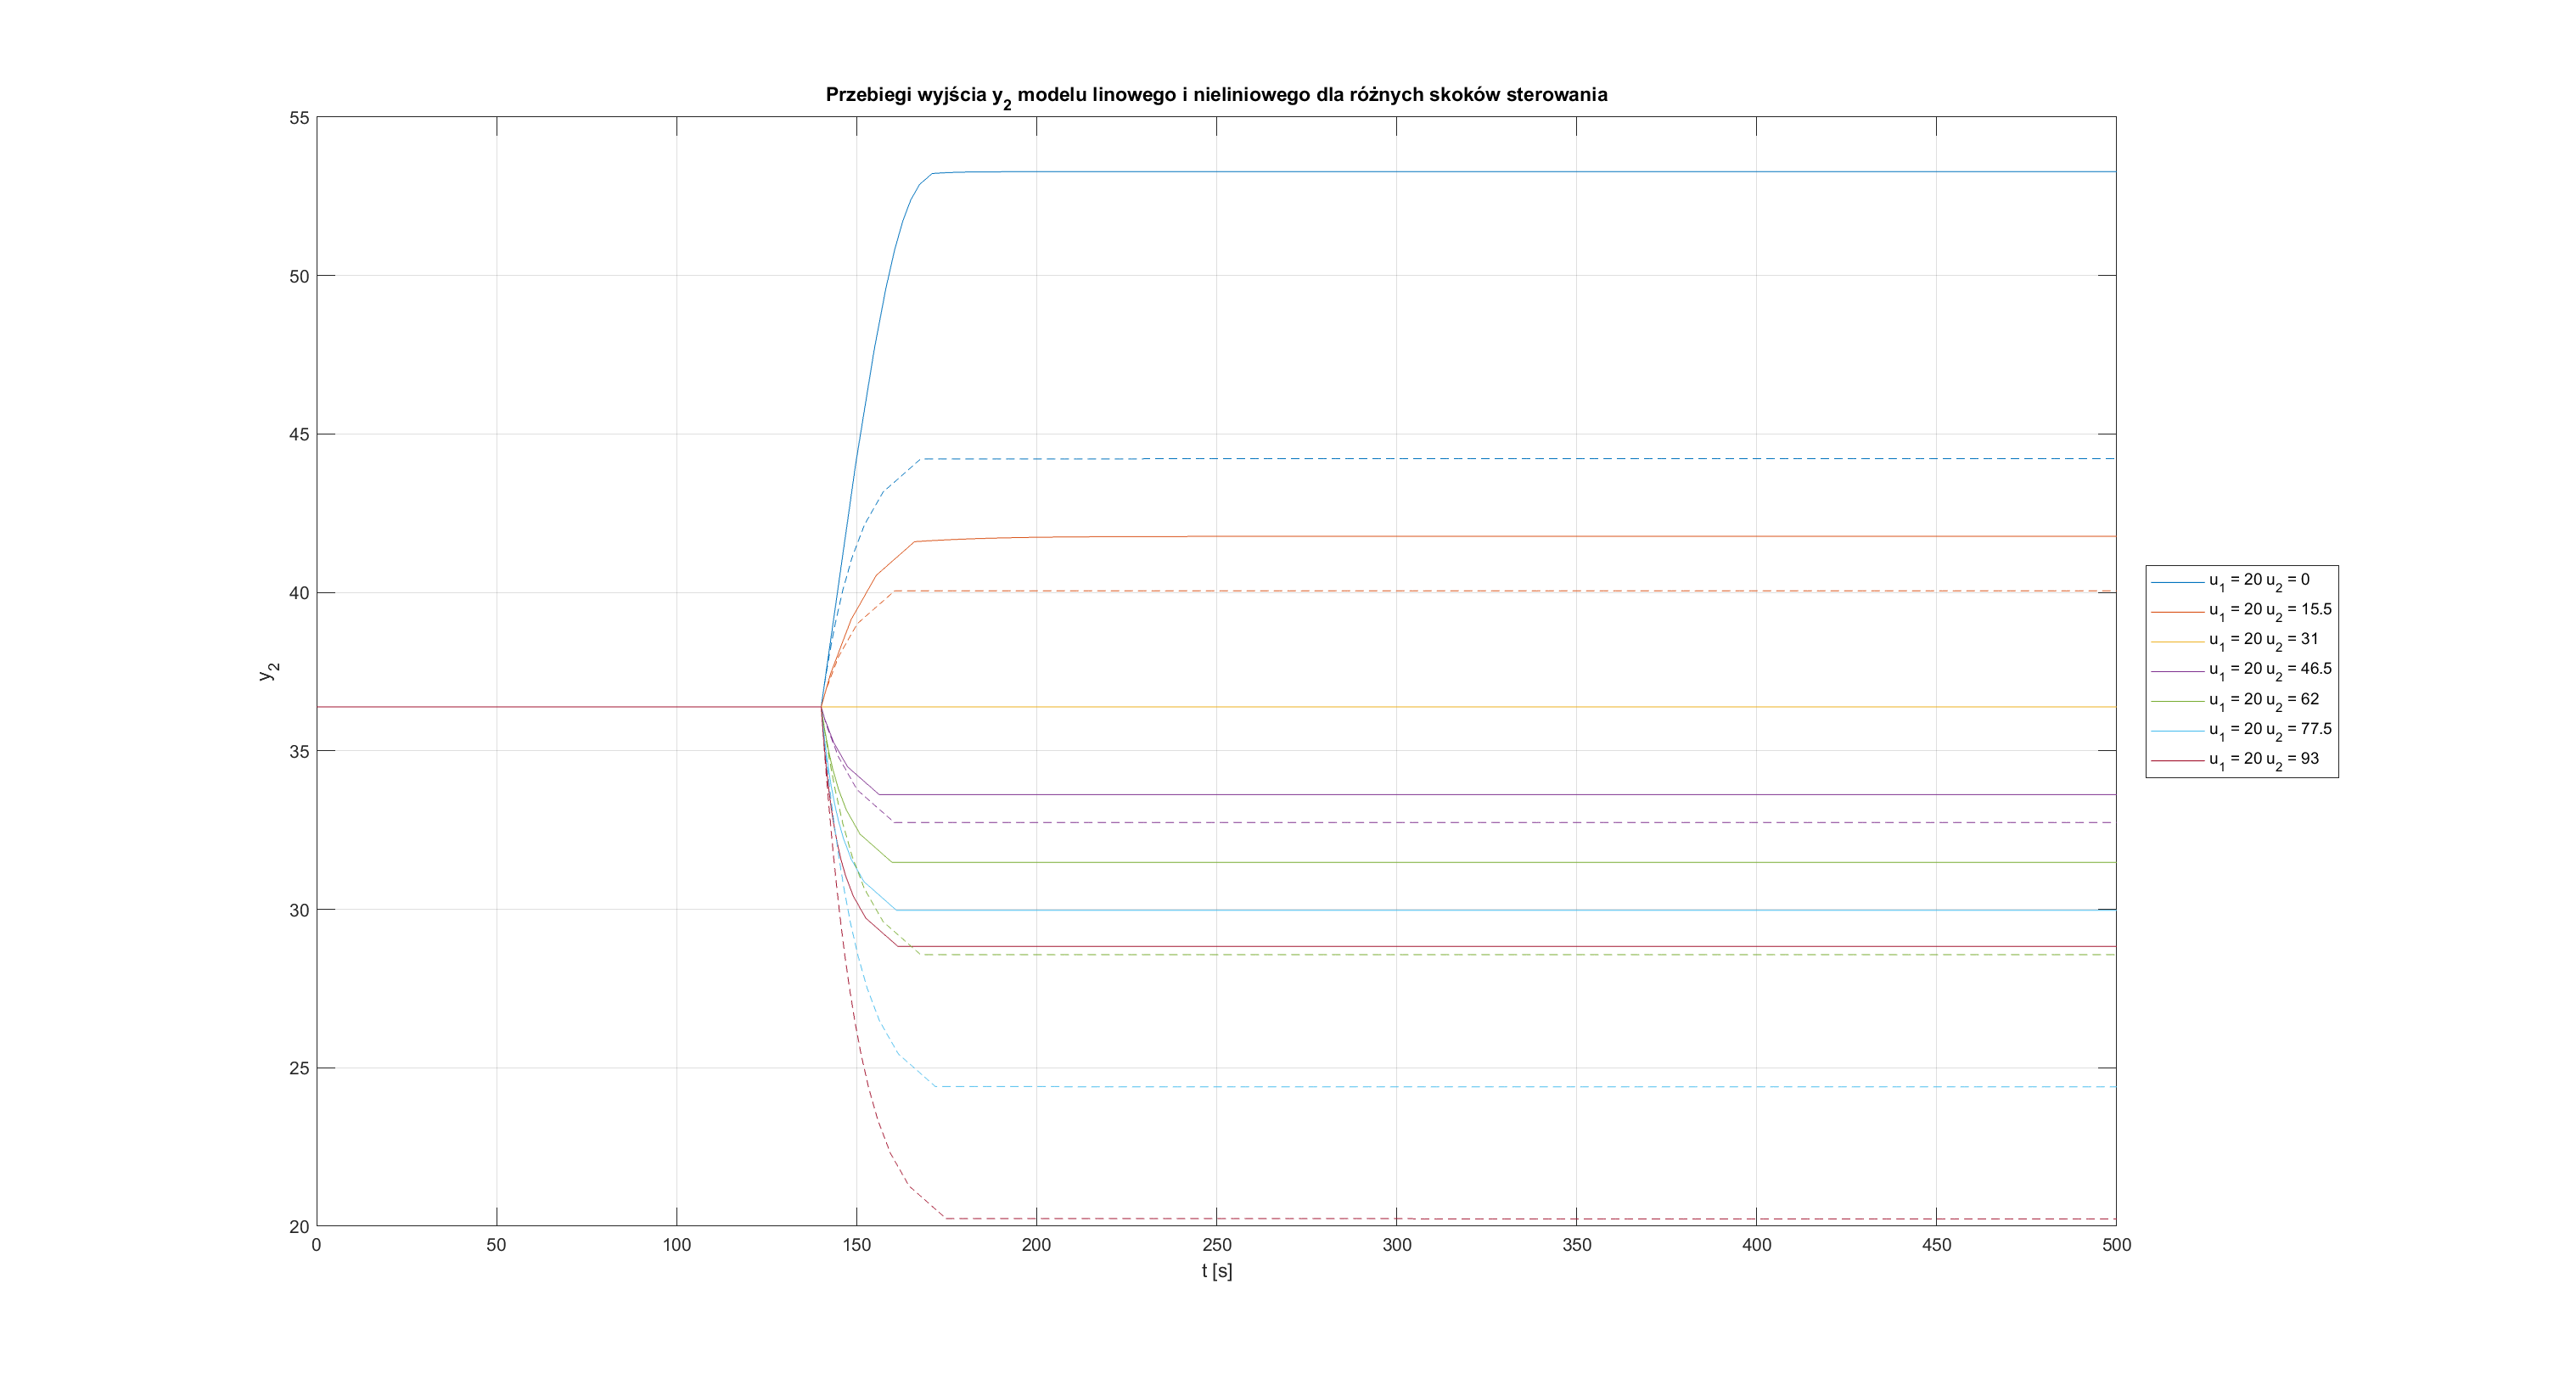
\includegraphics[scale=0.35]{images/y2_u1=20_u2=93_dt=0.1.eps}
    \caption{Porównanie modeli liniowych i nieliniowych}
\end{figure}

Dalej sprawdzono zachowanie układu przy zmianach wejścia zakłócającego $v_1$.

\begin{figure}[H]
    \centering
    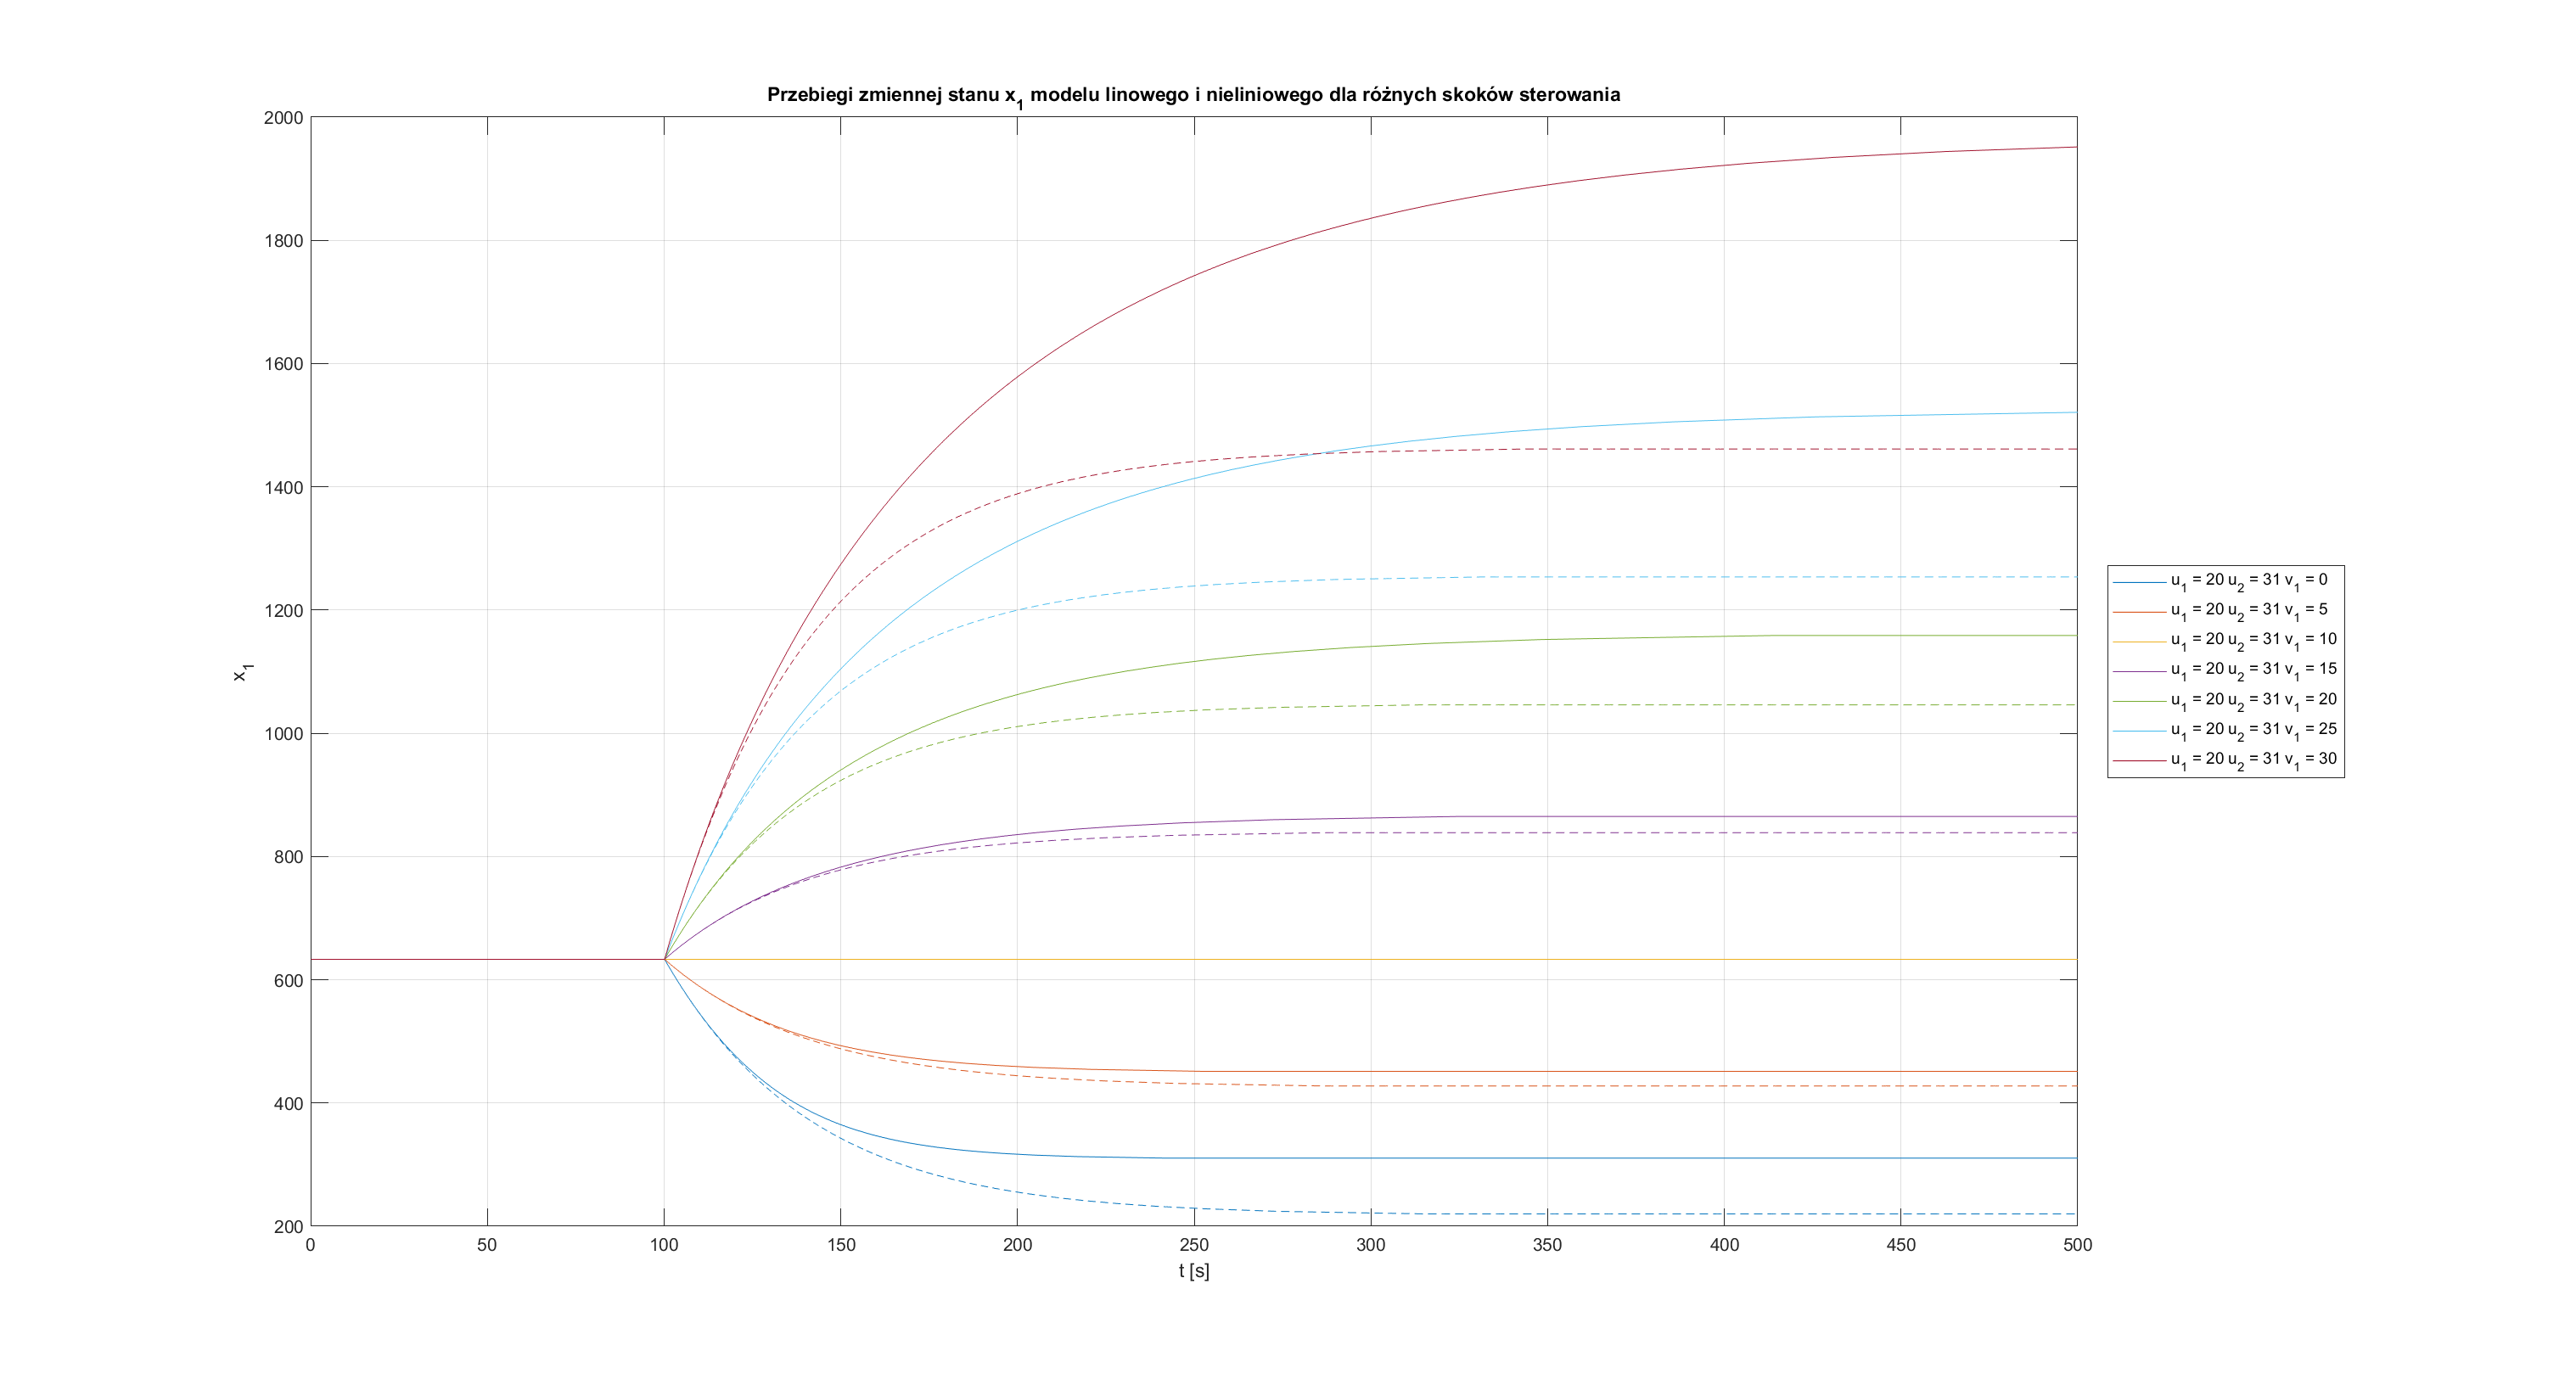
\includegraphics[scale=0.35]{images/x1_u1=20_u2=31_v1=30_dt=0.1.eps}
    \caption{Porównanie modeli liniowych i nieliniowych}
\end{figure}

\begin{figure}[H]
    \centering
    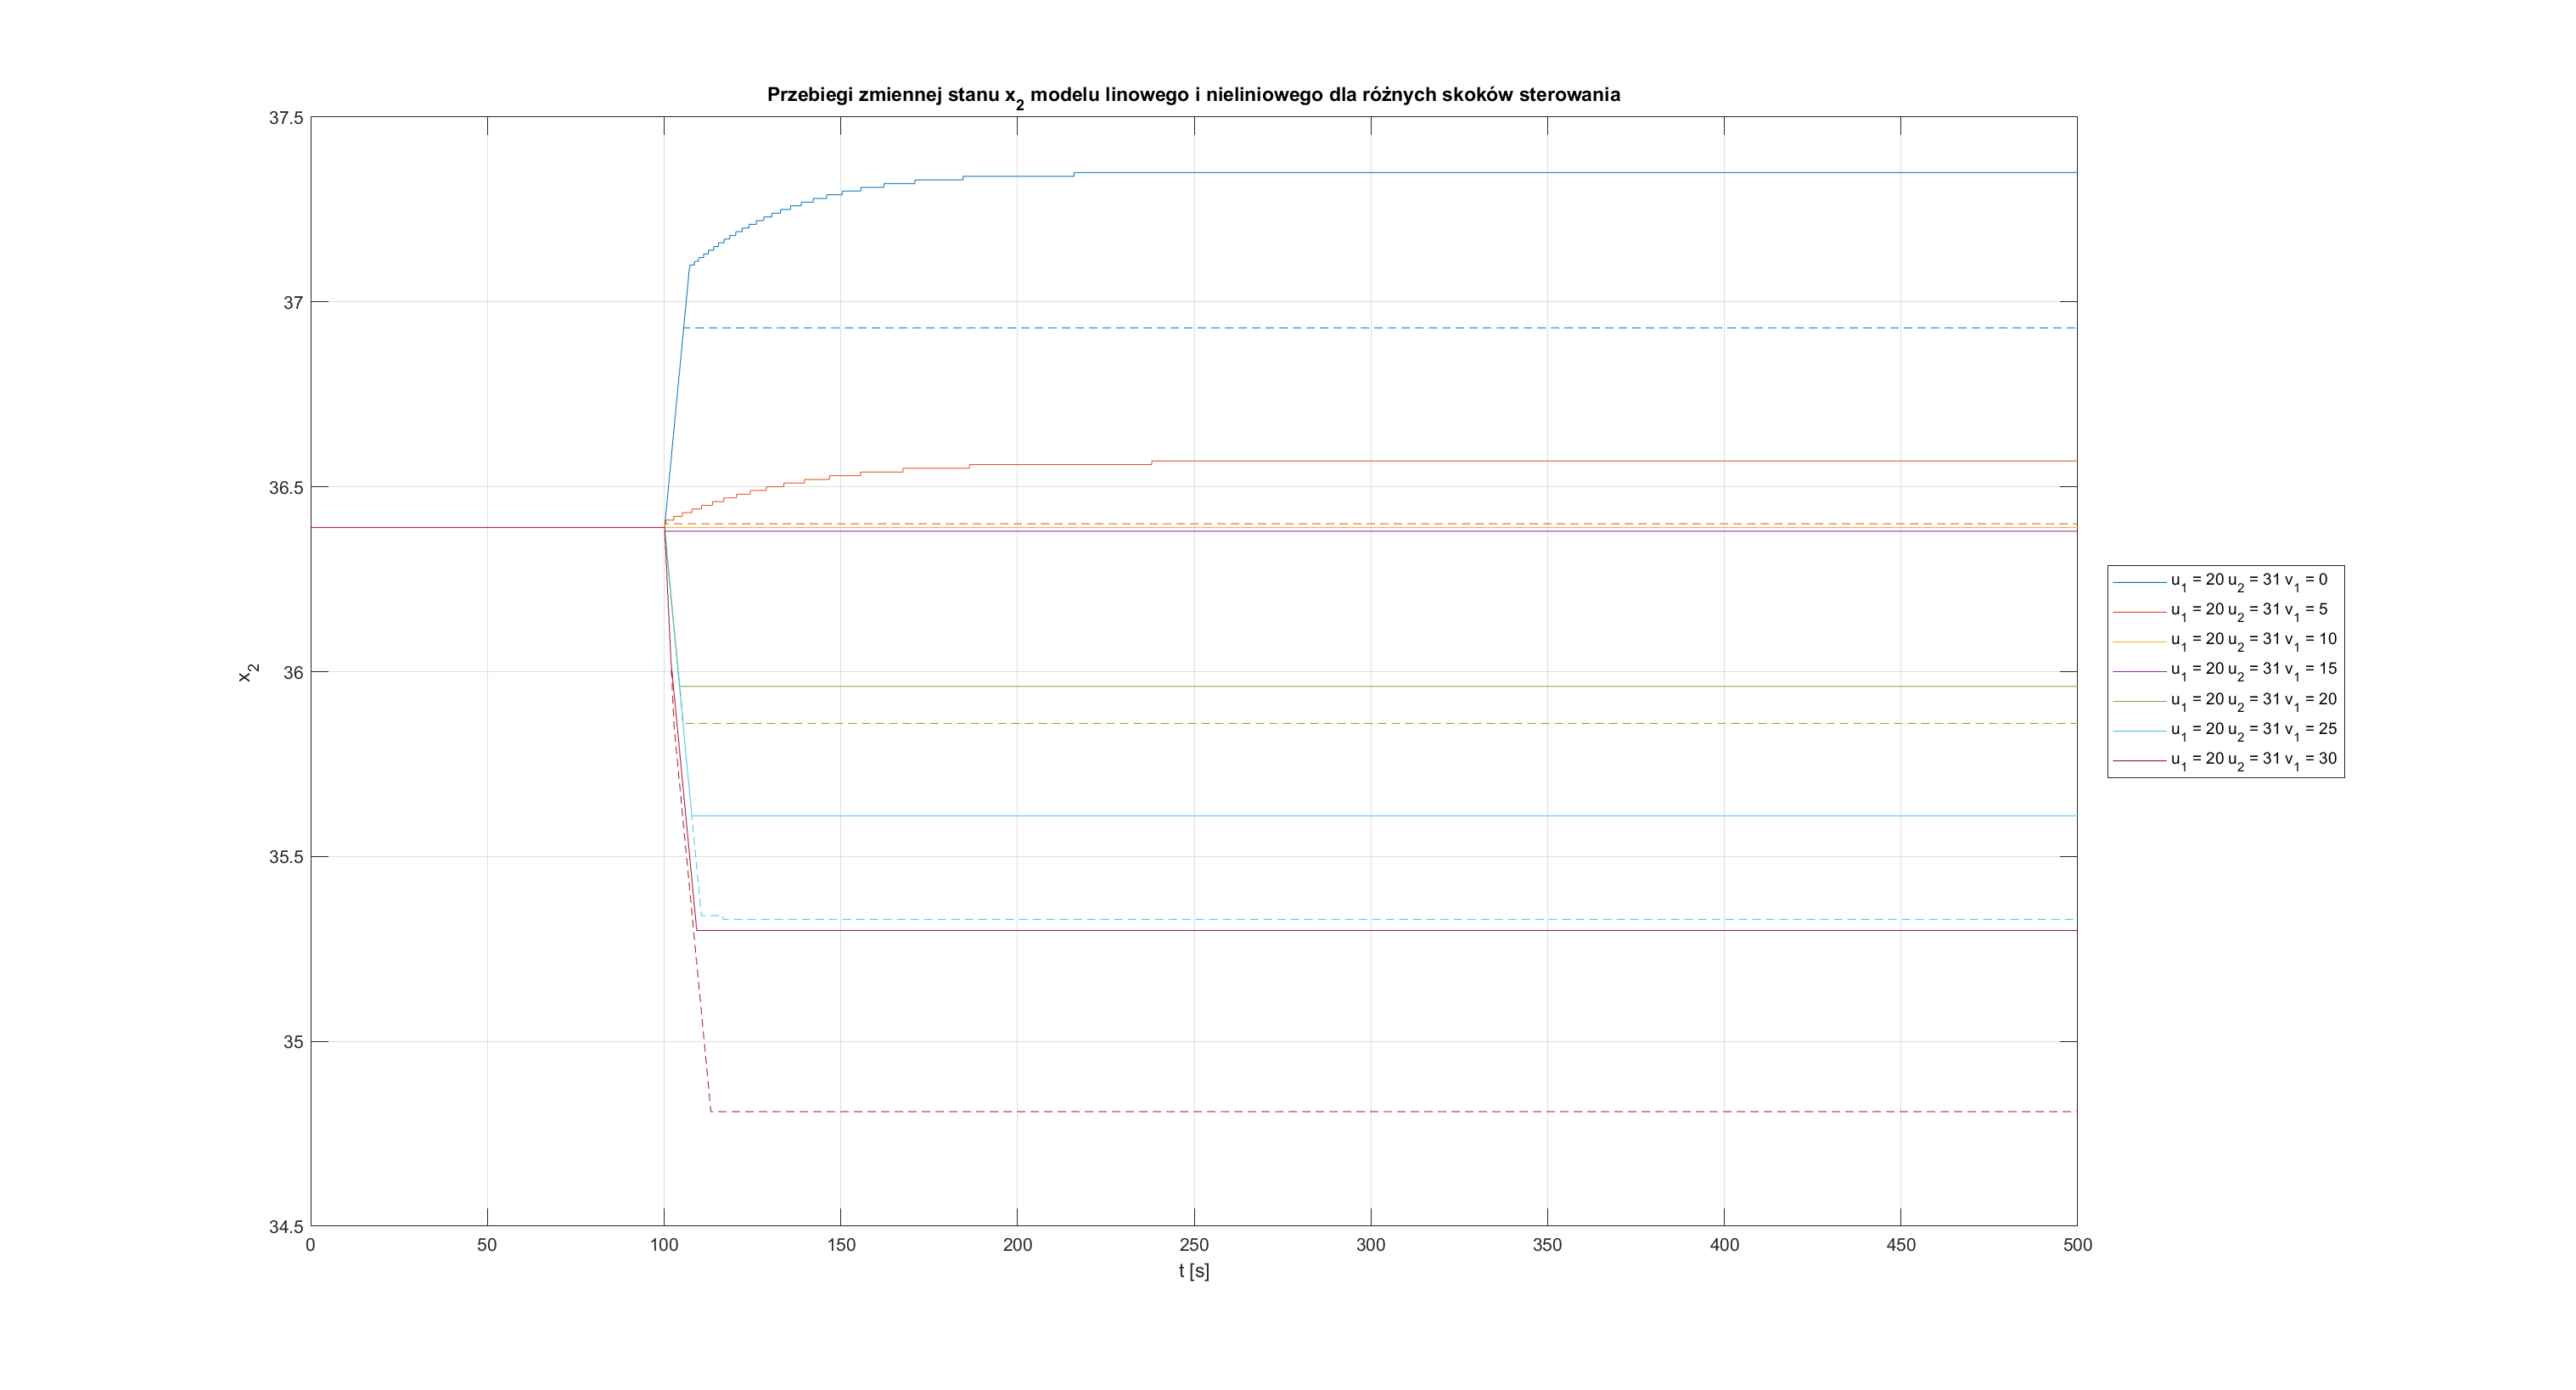
\includegraphics[scale=0.35]{images/x2_u1=20_u2=31_v1=30_dt=0.1.eps}
    \caption{Porównanie modeli liniowych i nieliniowych}
\end{figure}

\begin{figure}[H]
    \centering
    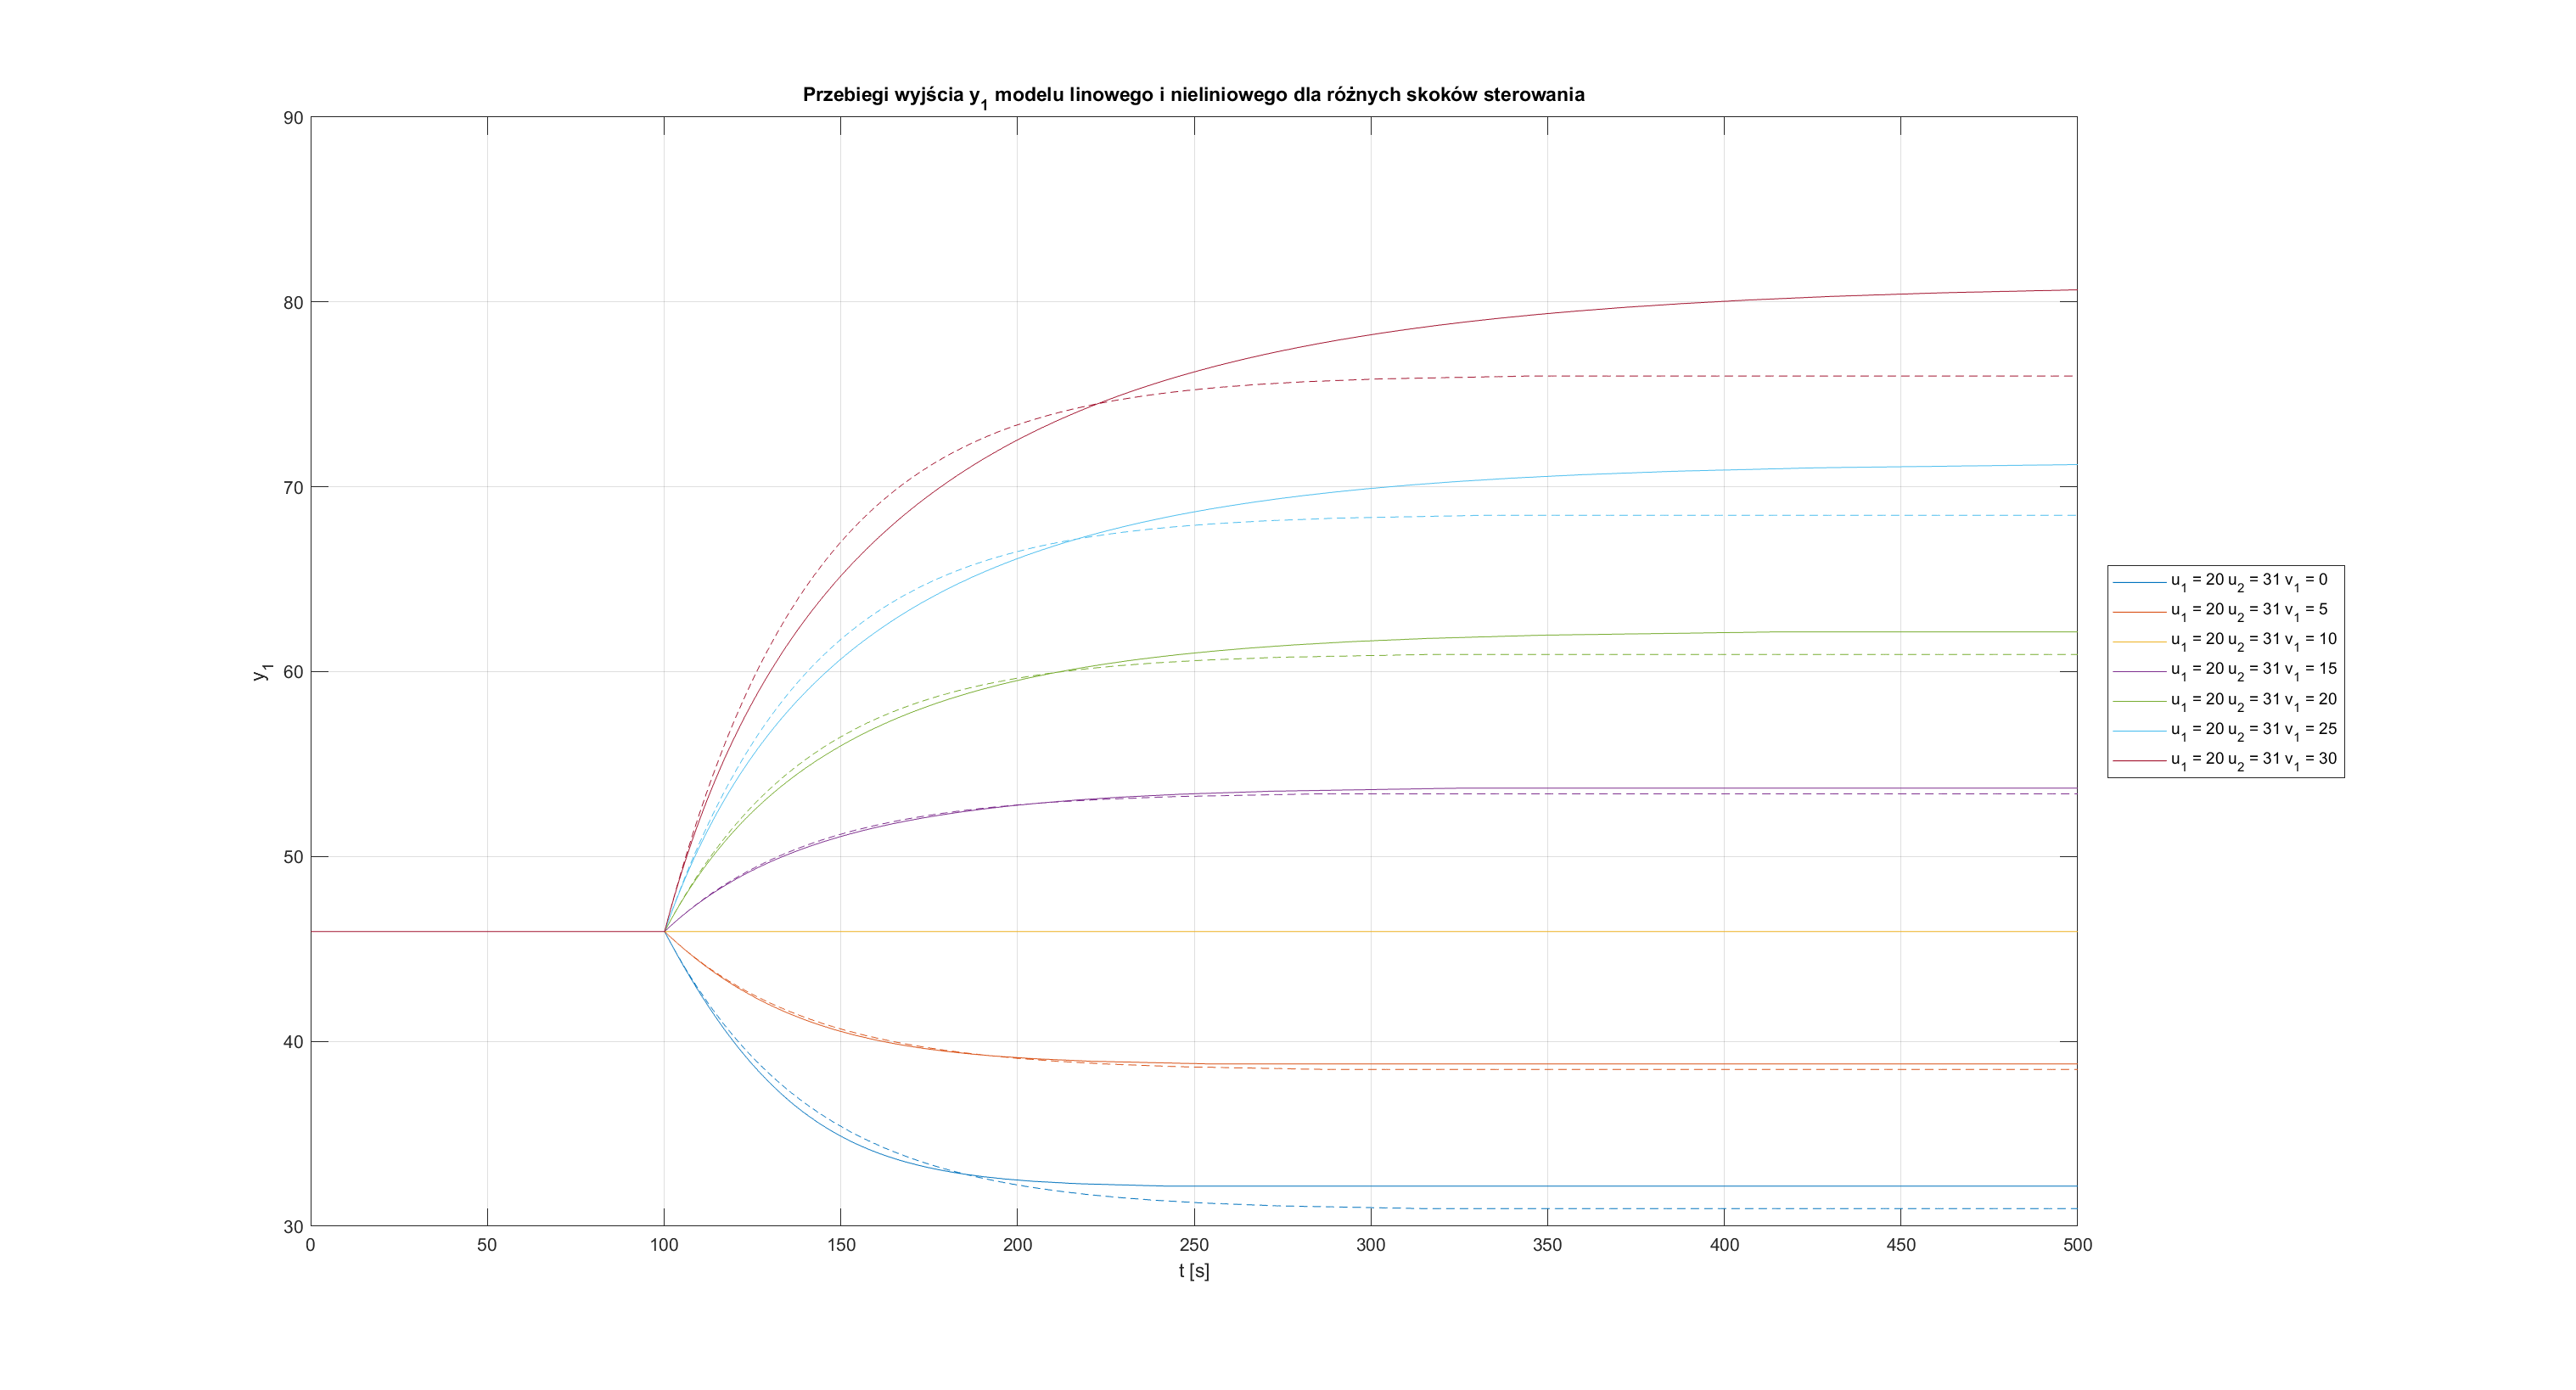
\includegraphics[scale=0.35]{images/y1_u1=20_u2=31_v1=30_dt=0.1.eps}
    \caption{Porównanie modeli liniowych i nieliniowych}
\end{figure}

\begin{figure}[H]
    \centering
    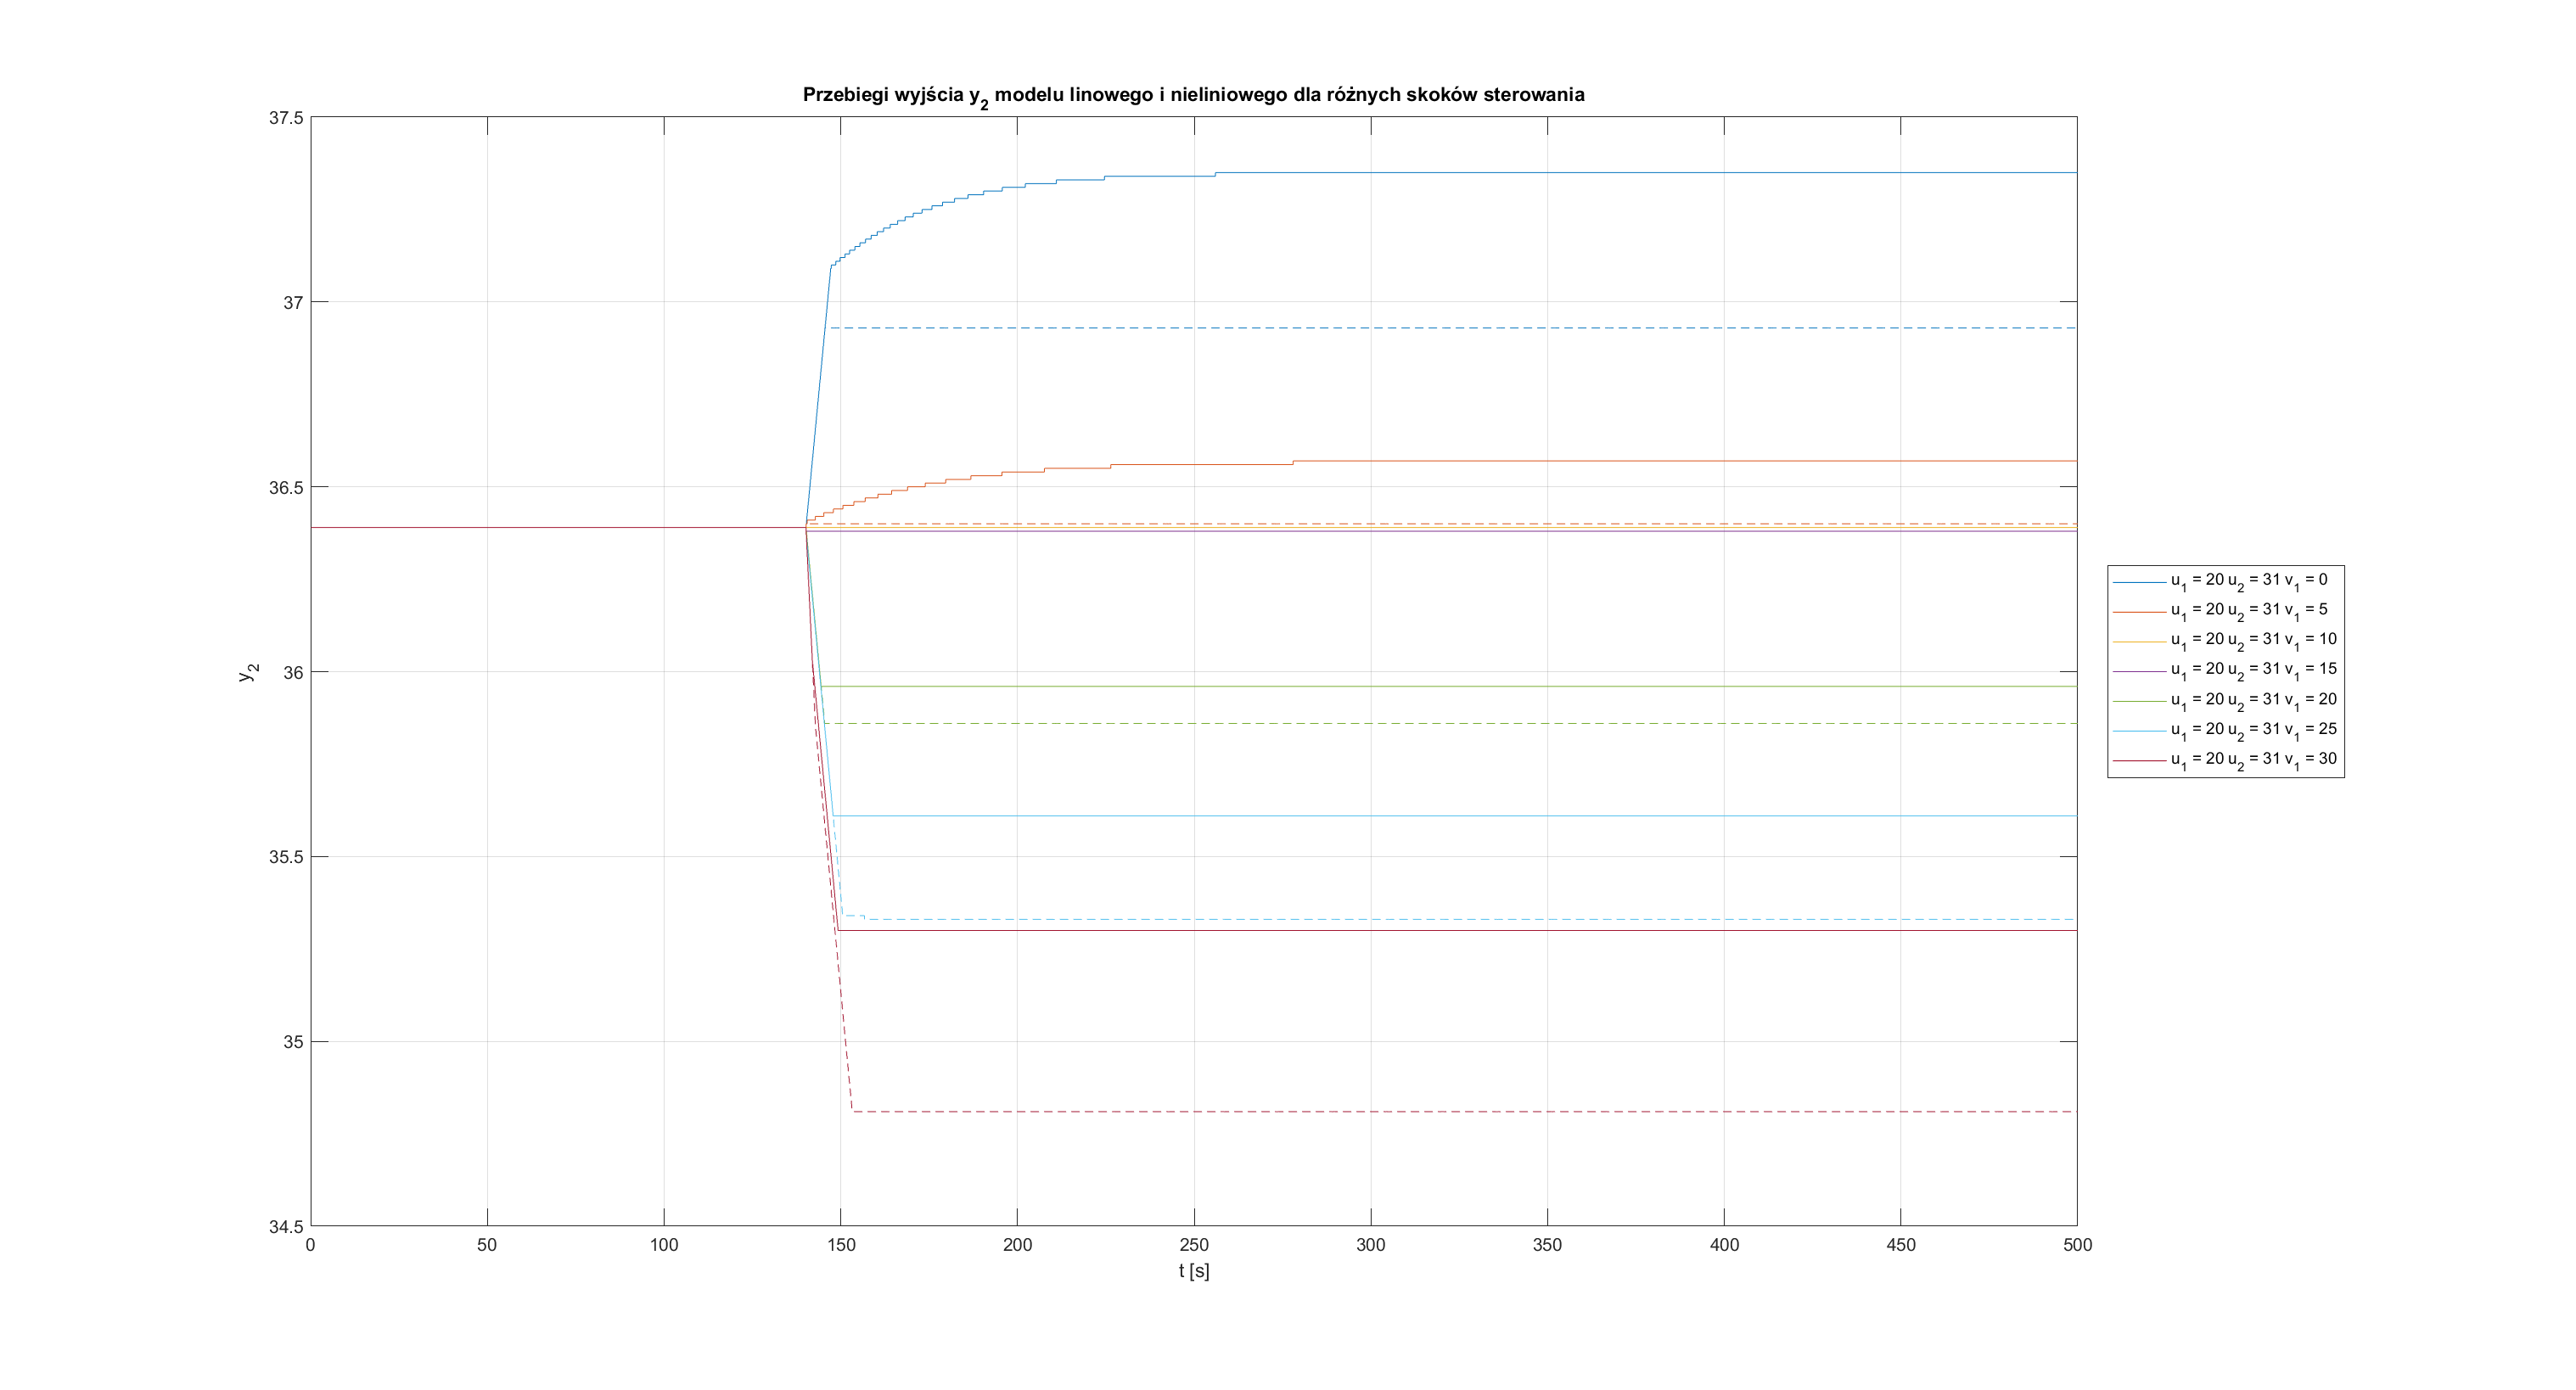
\includegraphics[scale=0.35]{images/y2_u1=20_u2=31_v1=30_dt=0.1.eps}
    \caption{Porównanie modeli liniowych i nieliniowych}
\end{figure}

W ostatnim eksperymencie zmieniano wszystkie wejścia naraz.

\begin{figure}[H]
    \centering
    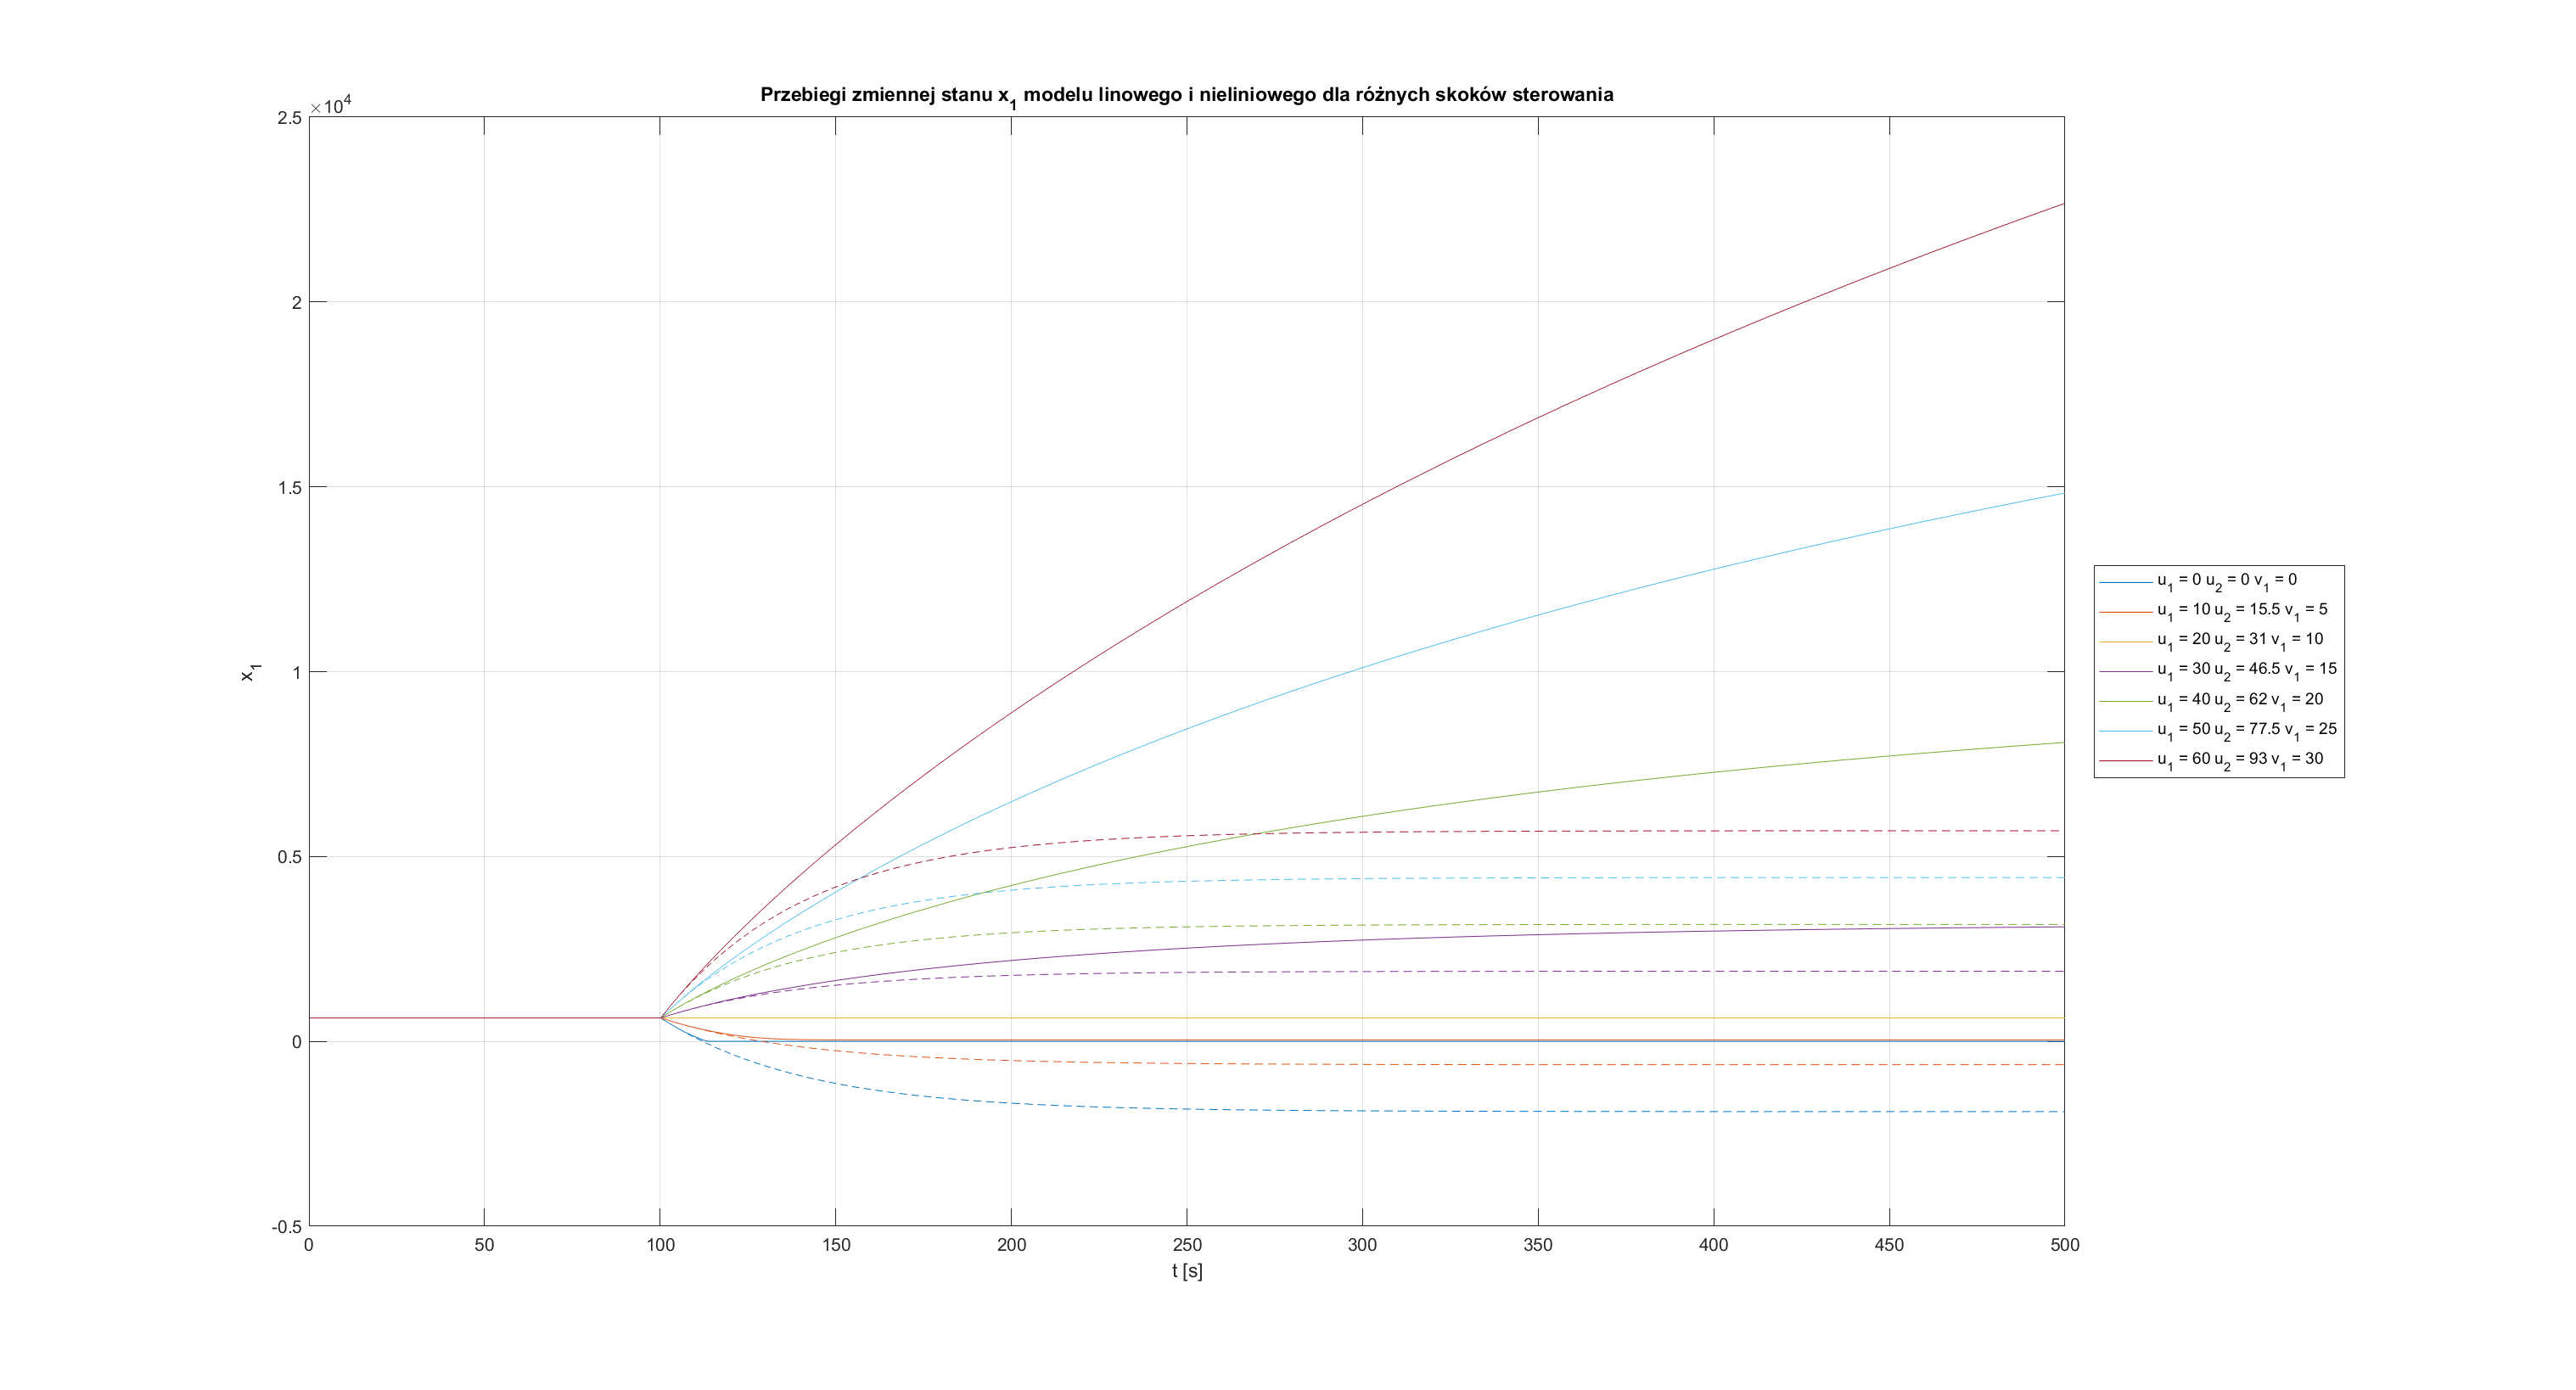
\includegraphics[scale=0.35]{images/x1_u1=60_u2=93_v1=30_dt=0.1.eps}
    \caption{Porównanie modeli liniowych i nieliniowych}
\end{figure}

\begin{figure}[H]
    \centering
    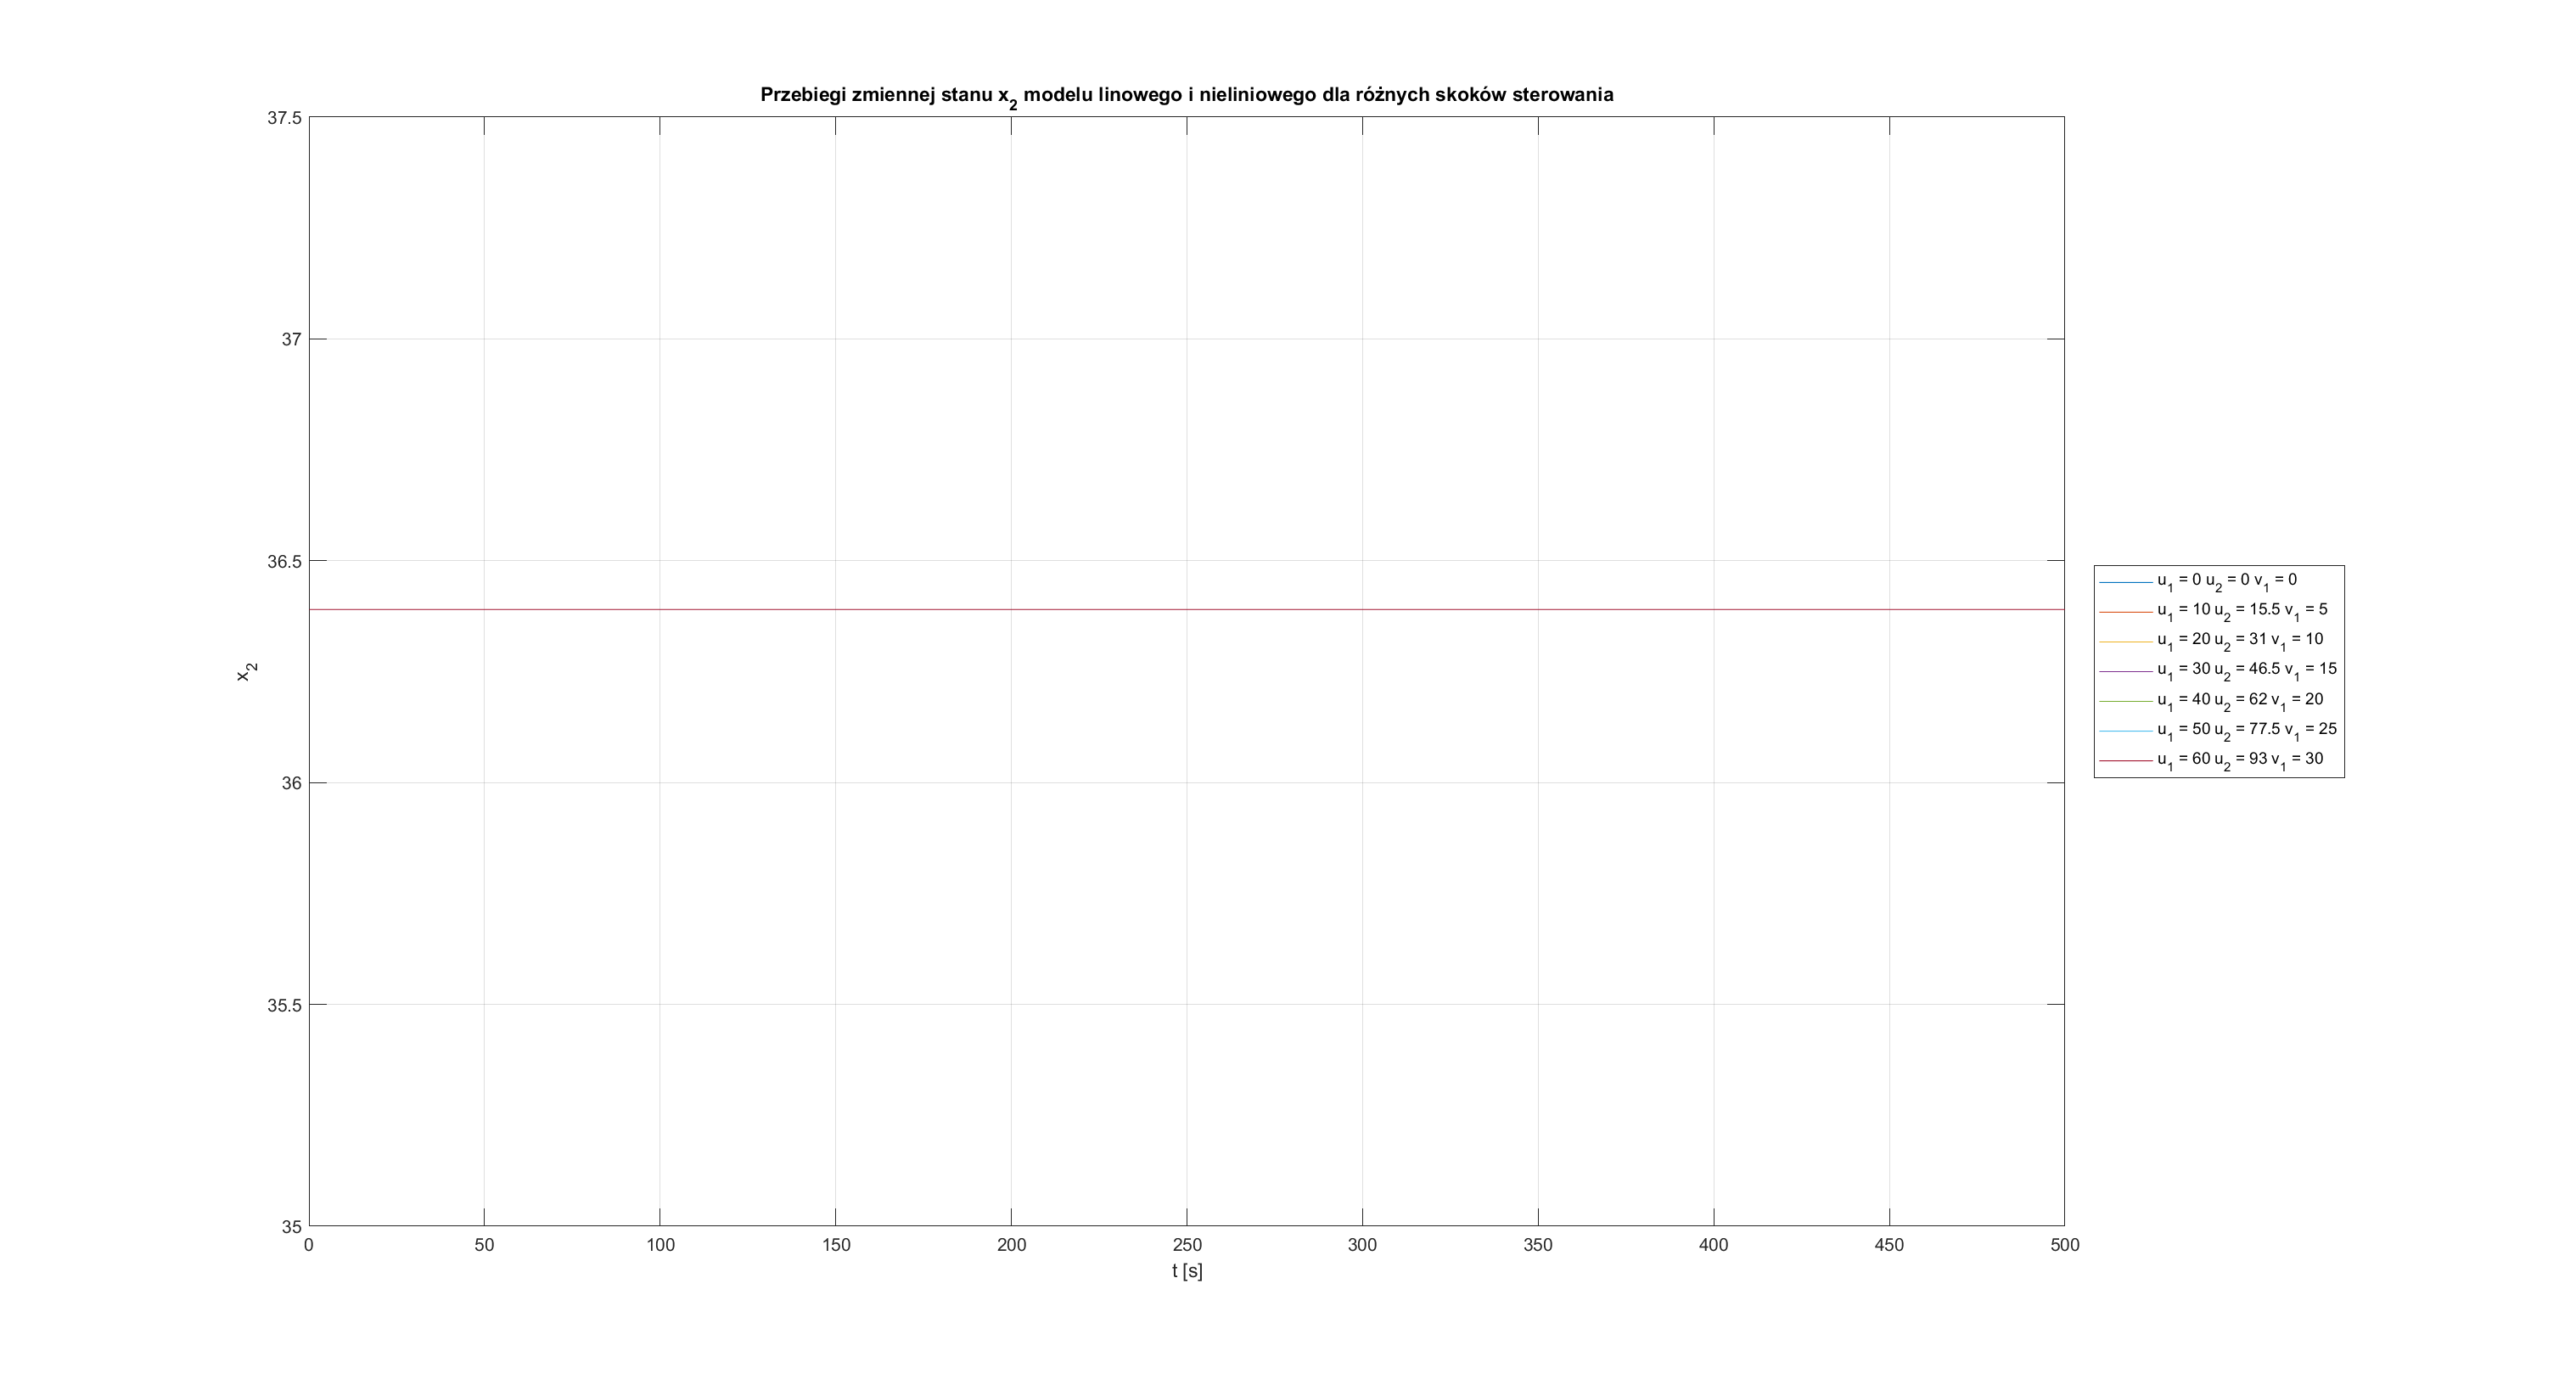
\includegraphics[scale=0.35]{images/x2_u1=60_u2=93_v1=30_dt=0.1.eps}
    \caption{Porównanie modeli liniowych i nieliniowych}
\end{figure}

\begin{figure}[H]
    \centering
    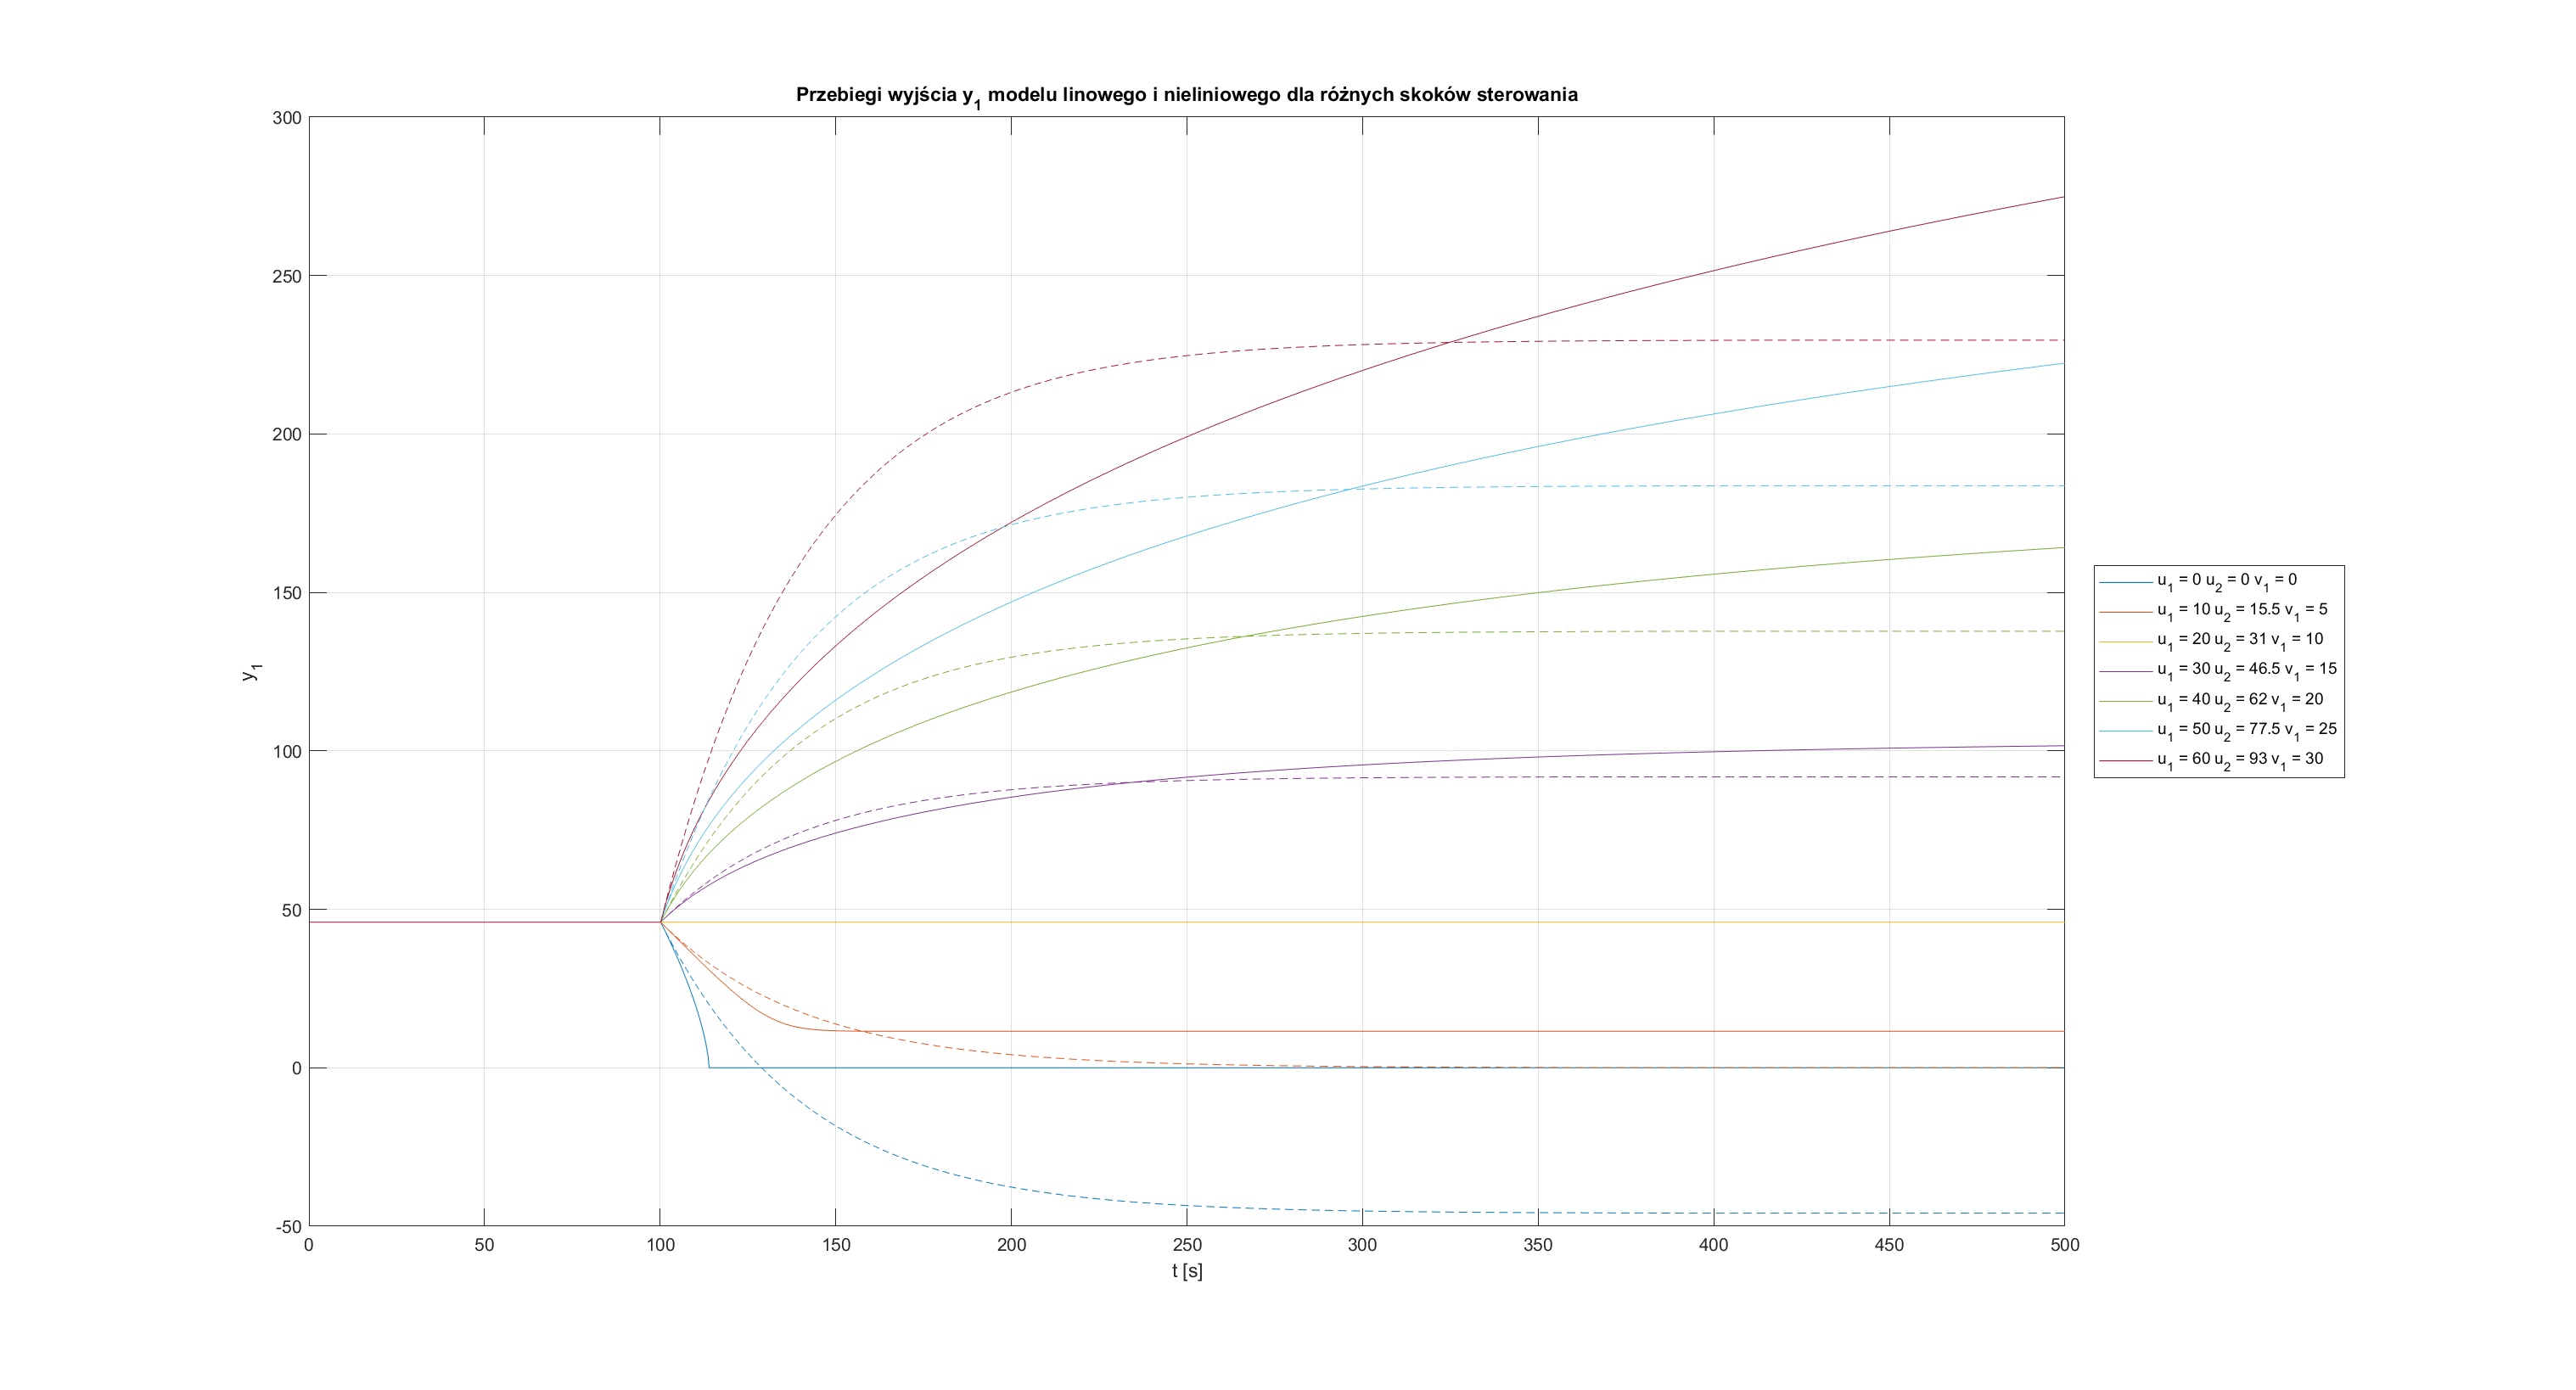
\includegraphics[scale=0.35]{images/y1_u1=60_u2=93_v1=30_dt=0.1.eps}
    \caption{Porównanie modeli liniowych i nieliniowych}
\end{figure}

\begin{figure}[H]
    \centering
    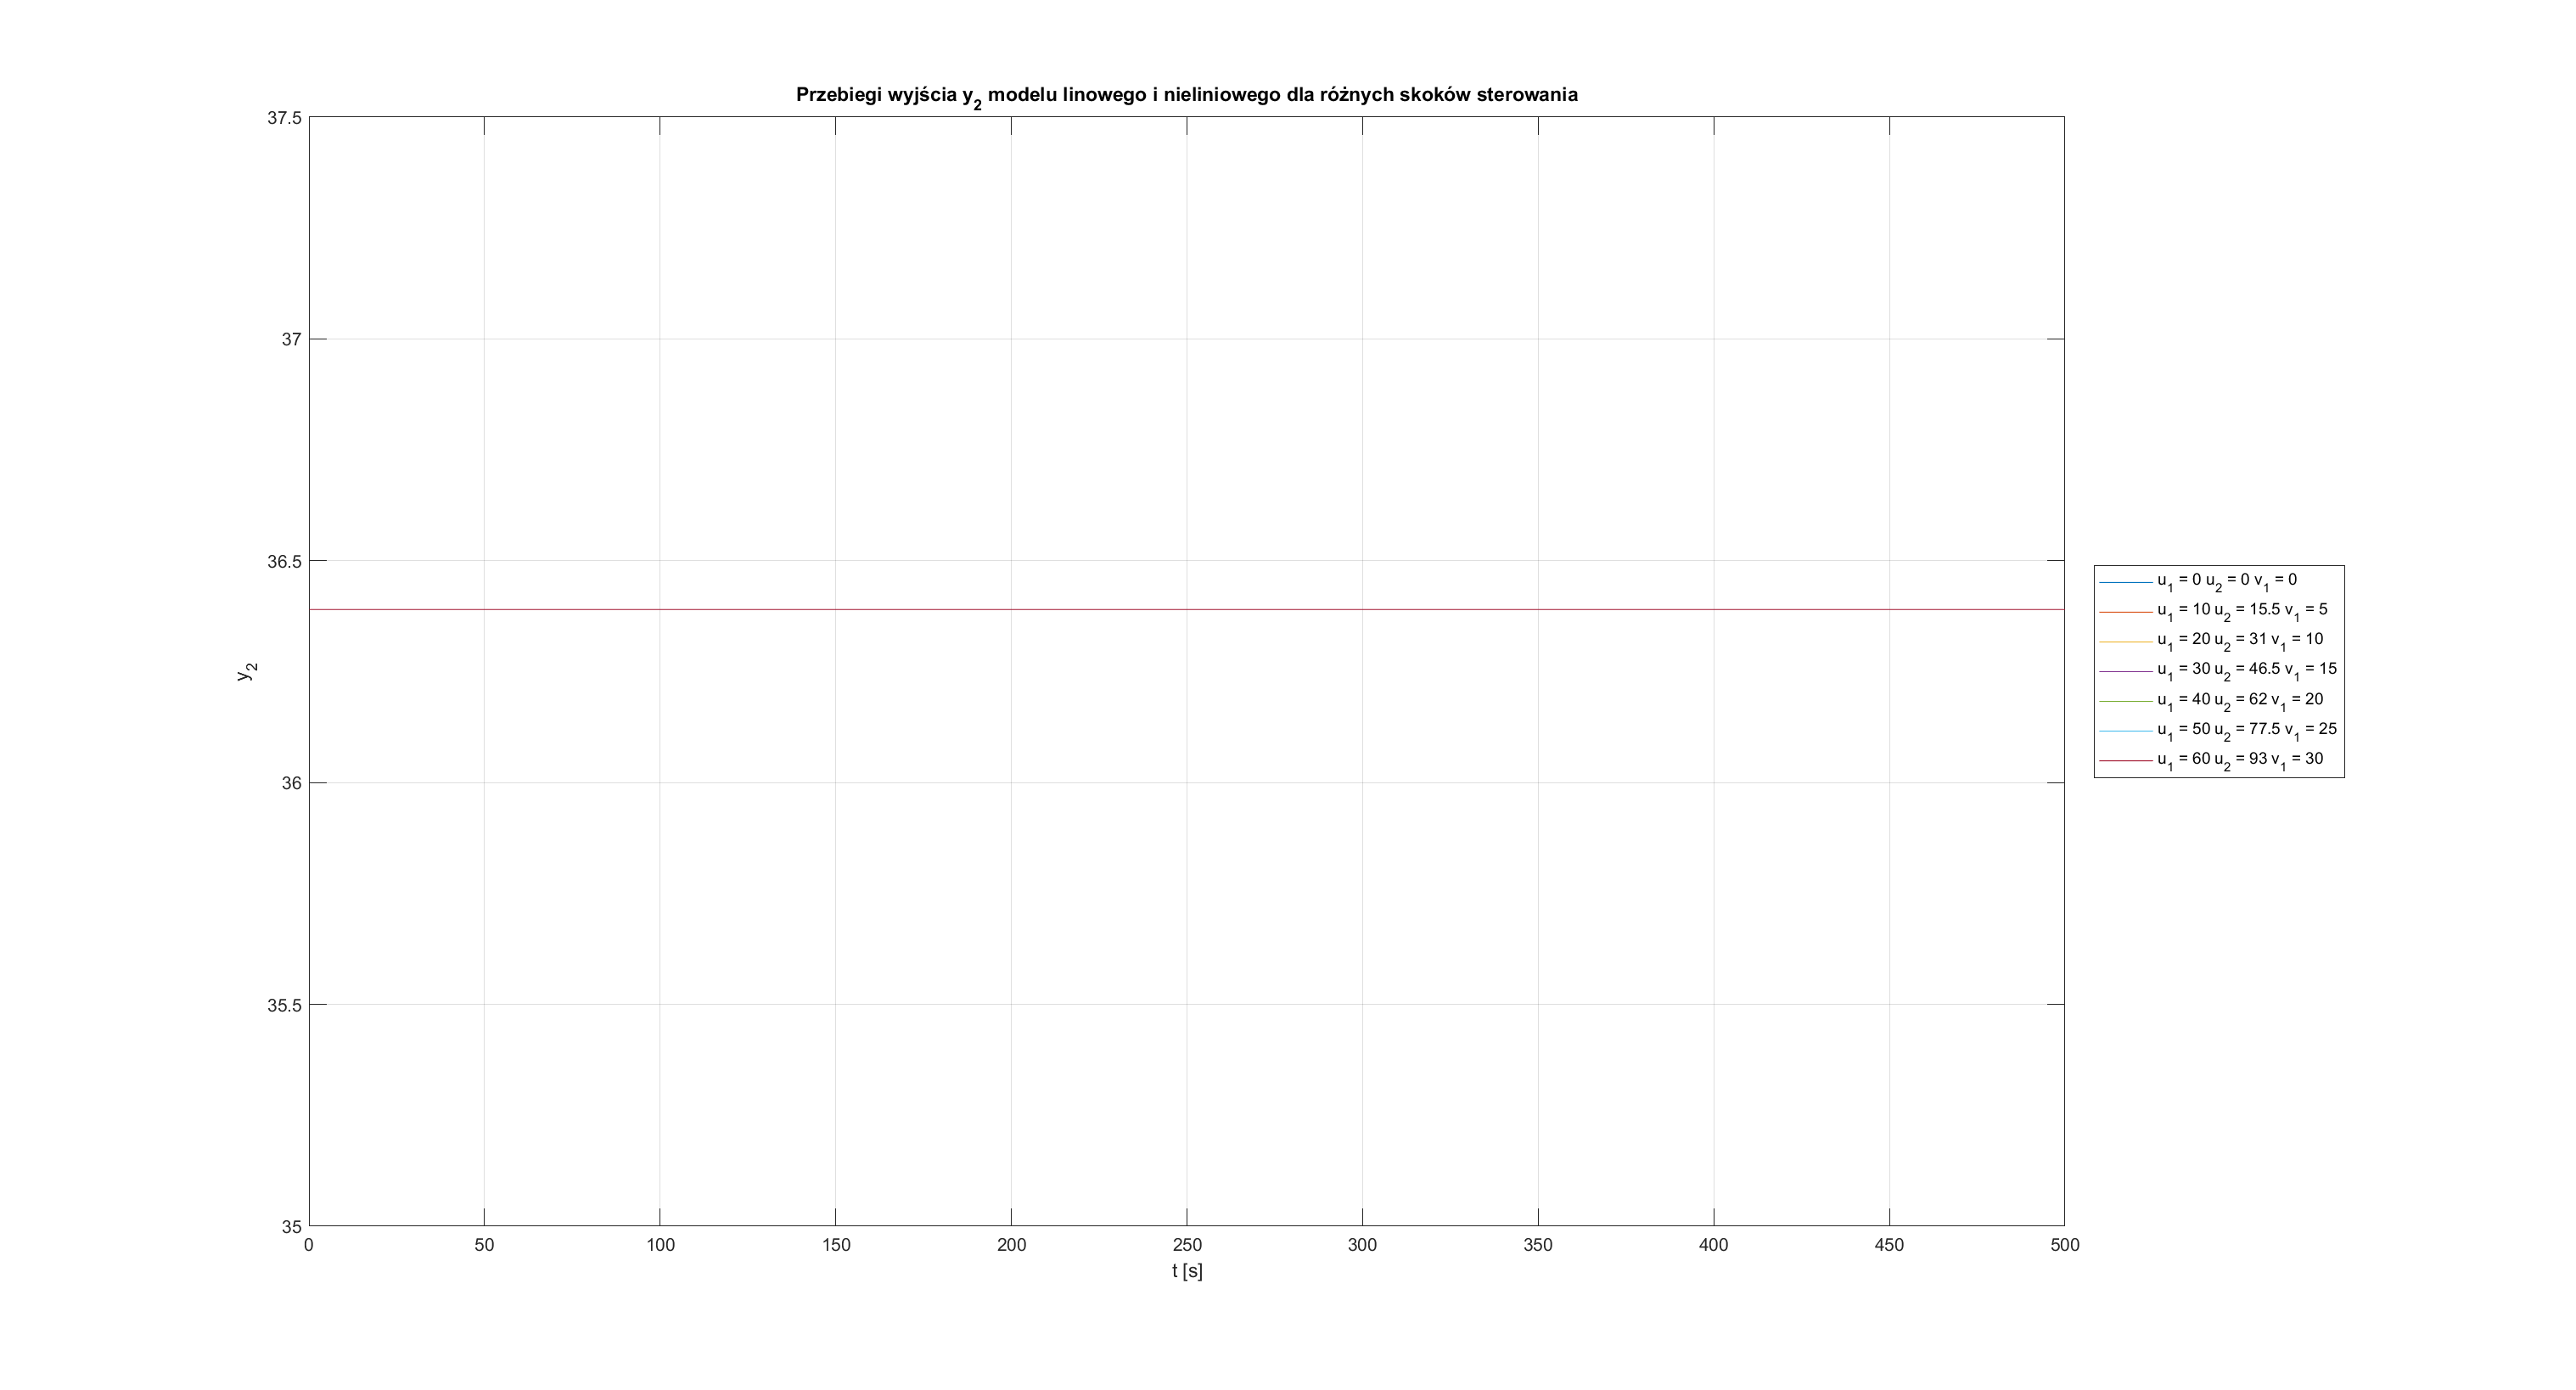
\includegraphics[scale=0.35]{images/y2_u1=60_u2=93_v1=30_dt=0.1.eps}
    \caption{Porównanie modeli liniowych i nieliniowych}
\end{figure}

Wniosek:
Wraz z oddaleniem się wejść oraz zakłócenia od parametrów zadanych przybliżenie modelu modelem liniowym stopniowo traci sens, gdyż wyniki zbyt znacząco się rozbiegają.